% ------------------------------------------------------------------------
% ------------------------------------------------------------------------
% Modelo de Trabalho Acadêmico utilizando repUERJ 
% tese de doutorado, dissertação de mestrado e trabalhos monográficos em geral
%
% * Este aquivo está editado na codificação de caracteres UTF-8.
%
% ------------------------------------------------------------------------
% ------------------------------------------------------------------------
%
\documentclass[a4paper,12pt,oneside,onecolumn,final,fleqn]{repUERJ}

% ---
% Pacotes fundamentais 
% ---
\usepackage[brazil]{babel}  % adequacao para o portugues Brasil
\usepackage[utf8]{inputenc} % Determina a codificacao utiizada
                            % (conversão automática dos acentos)
\usepackage{makeidx}        % Cria o indice
\usepackage{hyperref}       % Controla a formacao do indice
\usepackage{lastpage}       % Usado pela Ficha catalografica
\usepackage{indentfirst}    % Indenta o primeiro paragrafo de cada secao.
\usepackage{xcolor}          % Controle das cores
\usepackage{graphicx}       % Inclusao de graficos
\usepackage{subfig}
\usepackage{amsmath}        % pacote matemático
\usepackage{amssymb}
\usepackage{amsthm}
\usepackage{hhline}
\usepackage{tikz}
\usetikzlibrary{calc}
\usepackage{multirow}
\usepackage{bigstrut}
\usepackage{algpseudocode}

\usepackage{setspace}
\usepackage{caption}
\captionsetup[table]{singlelinecheck=false}
\captionsetup[figure]{slc=off}
\captionsetup{font=singlespacing}
\captionsetup{tableposition=top}

\theoremstyle{plain}
\newtheorem{thm}{Theorem}[chapter] % reset theorem numbering for each chapter

\theoremstyle{definition}
\newtheorem{defn}[thm]{Definition} % definition numbers are dependent on theorem numbers
\newtheorem{exmp}[thm]{Example}

\usepackage{macrosfabbri-basic}
\usepackage{macrosfabbri-dg}
\newcommand{\RNum}[1]{\uppercase\expandafter{\romannumeral #1\relax}}
\newcommand{\rnum}[1]{\expandafter{\romannumeral #1\relax}}
\renewcommand{\myparagraph}{\noindent\textbf}

% ---
% Pacote auxiliar para as normas da UERJ
% ---
\usepackage[frame=no,algline=yes,font=default]{repUERJformat}
% ---
% Pacotes de citacoes
% ---
\usepackage[alf]{abntex2cite}

% *****************************************************************************
% *****************************************************************************
% Comandos especificos deste exemplo 
% * podem ser retirados na edicao de um novo documento
% *****************************************************************************
% *****************************************************************************

\newcommand{\comando}[1]{\texttt{\bs #1}}
\newcommand{\opcoes}[1]{\texttt{[}\textsl{#1}\texttt{]}}
\newcommand{\param}[1]{\texttt{\{}\textsl{#1}\texttt{\}}}
\newcommand{\BibTeX}{{{Bib}}\TeX}
\newcommand{\repUERJ}{\textsf{repUERJ}}
\newcommand{\formato}[1]{\begin{flushleft}{#1}\end{flushleft}}
\newcommand{\bs}{\textbackslash}
\def\ReduceAfterCaptionfigspace{}

% *****************************************************************************
% *****************************************************************************
% Informacoes de autoria e institucionais
% *****************************************************************************
% *****************************************************************************

%-----------------------------------------------------------------------
% Imagens pretextuais (precisam estar no mesmo diretorio deste arquivo .tex)
%-----------------------------------------------------------------------

\logo{logo_uerj_cinza.png}
\marcadagua{marcadagua_uerj_cinza.png}{1}{160}{255}
%-----------------------------------------------------------------------
% Informacoes da instituicao
%-----------------------------------------------------------------------

\instituicao{Universidade do Estado do Rio de Janeiro}
            {Instituto Politécnico} 
            {Departamento de Modelagem Computacional}  
            {}

%-----------------------------------------------------------------------
% Informacoes da autoria do documento
%-----------------------------------------------------------------------

\autor{Pedro Felipe Pena}{Barata}
\titulo{Aplicações de técnicas atuais em reconstrução 3D fotogramétrica}

\palavraschaves{Fotogrametria}{VisualSfM}{MVE -- \emph{Multi-View Reconstruction Environment}}{Reconstrução 3D}

\title{Applications of current photogrammetric 3D reconstruction techniques}
\keywords{Photogrammetry}{VisualSfM}{MVE -- Multi-View Reconstruction Environment}{3D Reconstruction}

\orientador{Prof.\ Dr.} 
           {Ricardo}{Fabbri} 
           {Departamento de Modelagem Computacional -- UERJ}

%-----------------------------------------------------------------------
% Titulacao (Doutor, Mestre, Bacharel, Licenciado) e Curso
%-----------------------------------------------------------------------

\grau{Graduado}  
\curso{Engenharia de Computação} 
\areadeconcentracao{}

%-----------------------------------------------------------------------
% Informacoes adicionais (local, data e paginas)
%-----------------------------------------------------------------------

\local{Nova Friburgo} 
\data{23}{Novembro}{2017} 

% *****************************************************************************
% *****************************************************************************
% Configurações de aparência do PDF final
% *****************************************************************************
% *****************************************************************************

% alterando o aspecto da cor azul
\definecolor{blue}{RGB}{41,5,195}
\definecolor{apricot}{RGB}{251,206,177}

% informações do PDF
\hypersetup{
  %backref=true,
  %pagebackref=true,
  %bookmarks=true,                  % show bookmarks bar?
  unicode=false,
  pdftitle={\UERJtitulo},
  pdfauthor={\UERJautor},
  pdfsubject={\UERJpreambulo},
  pdfkeywords={PALAVRAS}{CHAVES}{\chaveA}{\chaveB}{\chaveC}{\chaveD},
  pdfproducer={\packagename}, % producer of the document
  pdfcreator={\UERJautor},
  colorlinks=true,                  % false: boxed links; true: colored links
  linkcolor=blue,                   % color of internal links blue
  citecolor=red,                    % color of links to bibliography blue
  filecolor=magenta,                % color of file links magenta
  urlcolor=green,
  bookmarksdepth=4
}

% *****************************************************************************
% *****************************************************************************
% Início do documento
% *****************************************************************************
% *****************************************************************************

% ---
% compila o indice
% ---
\makeindex
% ---

% *****************************************************************************
% *****************************************************************************

\begin{document}
\pagestyle{empty}
\begin{tikzpicture}[overlay,remember picture]
    \draw [line width=2pt ]
        ($ (current page.north west) + (2cm,-2cm) $)
        rectangle
        ($ (current page.south east) + (-1cm,1.5cm) $);
    \draw [line width=1pt]
        ($ (current page.north west) + (2.1cm,-2.1cm) $)
        rectangle
        ($ (current page.south east) + (-1.1cm,1.6cm) $);
\end{tikzpicture}
% ----------------------------------------------------------
% ELEMENTOS PRE-TEXTUAIS
% ----------------------------------------------------------

\frontmatter

% ----------------------------------------------------------
% Capa e a folha de rosto
% ----------------------------------------------------------

\capa
\pagestyle{empty}
\begin{tikzpicture}[overlay,remember picture]
    \draw [line width=2pt ]
        ($ (current page.north west) + (2cm,-2cm) $)
        rectangle
        ($ (current page.south east) + (-1cm,1.5cm) $);
    \draw [line width=1pt]
        ($ (current page.north west) + (2.1cm,-2.1cm) $)
        rectangle
        ($ (current page.south east) + (-1.1cm,1.6cm) $);
\end{tikzpicture}

\folhaderosto % modelo de folha de rosto para monografia do Inst. Fís. UERJ

% ----------------------------------------------------------
% Inserir a ficha catalografica
% ----------------------------------------------------------

%\fichacatalografica{fichacatalografica.pdf}

% ----------------------------------------------------------
% Folha de aprovacao
% ----------------------------------------------------------

\begin{folhadeaprovacao}
  \assinatura{Prof. Dr. Edirlei Soares -- UERJ}
  \assinatura{Prof. Dr. Roberto Pinheiro -- UERJ}

\end{folhadeaprovacao}

% ----------------------------------------------------------
% Dedicatoria
% ----------------------------------------------------------

%\pretextualchapter{Dedicatória}

%\vfill

% ----------------------------------------------------------
% Agradecimentos
% ----------------------------------------------------------

\pretextualchapter{Agradecimentos}

A Deus por ter me dado saúde e força para superar as dificuldades.


Á minha família por sempre me apoiar, até nos momentos mais dificeis.


Á UERJ e todo seu corpo docente, além da direção e administração, que mesmo sem ter condições ideais de funcionamento, realizam seu trabalho com tanto amor e dedicação, trabalhando incansavelmente para que nós, alunos, possamos contar com um ensino de extrema qualidade.


Ao meu professor e orientador Ricardo Fabbri, pelo suporte no pouco tempo que lhe coube, pelas suas correções e incentivos.

% ----------------------------------------------------------
% Epigrafe
% ----------------------------------------------------------

\pretextualchapter{}

  \vfill\
  \begin{flushright}
 Talvez não tenha conseguido fazer o melhor, mas lutei para que o melhor fosse feito. Não sou o que deveria ser, mas Graças a Deus, não sou o que era antes. \\
    \textsl{Marthin Luther King}
  \end{flushright}

% ----------------------------------------------------------
% RESUMO
% ----------------------------------------------------------

\pretextualchapter{Resumo}

\referencia

A área de reconstrução 3D vem sido amplamente explorada. Sensores de
profundidade, tanto aéreos quanto terrestres, têm sido empregados em diferentes
aplicações já há muito tempo. Entretanto, constantes melhorias na tecnologia, sobretudo, no
\emph{hardware} e \emph{software} no âmbito da reconstrução, fizeram com que
nas últimas duas décadas, novas técnicas surgissem.

Muitos cientistas que utilizavam a fotogrametria pura -- isto é, usando apenas
imagens -- converteram seus esforços à área dos sensores à laser. Além de
executarem uma reconstrução mais rápida e confiável de objetos com baixa
textura, tais sensores possuem uma altíssima acurácia, compensando seu alto
custo inicial.  Isto dificultou e desacelerou o processo de descoberta de novos
algoritmos e métodos na área da fotogrametria pura.

Graças a avanços recentes, a fotogrametria, aliada a novos algoritmos,
como o \emph{Structure from Motion} (SfM), pontos de interesse e o casamento entre
imagens, por exemplo, consegue competir com scanners à laser e sensores de
profundidade. As características mais bem-reconhecidas das técnicas recentes, no
entanto, são a robustez, flexibilidade, e praticidade, não sendo claro se na prática podem 
competir com scanners à laser quanto à precisão em aplicações de interesse.

Neste trabalho, investiga-se a praticidade de técnicas atuais combinando SfM e MVS
(\emph{Multi-View Stereo}), utilizando \emph{softwares} como o MVE~\cite{mve} e
o VisualSfM~\cite{wu2011visualsfm}. Em particular, relata-se um estudo de até
onde é possível chegar apenas utilizando-se a câmera de um \emph{smartphone}, visando
aplicação futura à preservação completa do patrimônio do Jardim do Nêgo, em Nova Friburgo.
Essa tecnologia é confrontada com outros tipos de técnicas empregadas em
grandes projetos, como o Kinect, da Microsoft, e sua aplicação em SfM, bem como técnicas clássicas de 
escaneamento a laser, tais como as empregadas no projeto \emph{Digital Michaelangelo} de preservação de
esculturas liderado pela Universidade de Stanford.


% O trabalho foi estruturado da seguinte maneira: previamente apresentam-se os objetivos do projeto, destacando suas funcionalidades e metas, a seguir divide-se em capítulos; O Capítulo 1, que introduz o funcionamento de cada algoritmo e técnica empregada, apresentando e debatendo, comparativamente pontos à favor e contra; O Capítulo 2 é dedicado à ferramenta gráfica utilizada para a obtenção dos resultados (VisualSfM). Finalmente, apresentamos os resultados e conclusões do trabalho, bem como sugestões para implementações e trabalhos futuros.

% ABORDAR OS "TODO'S" DO HANGOUTS


\imprimirchaves

% ----------------------------------------------------------
% Abstract
% ----------------------------------------------------------

\pretextualchapter{Abstract}

\reference

The field of 3D reconstruction has been widely explored. Range sensors, both aerial
and terrestrial, have long been employed in different applications. However, constant
improvements in technology, especially in hardware and software in the context
of reconstruction, have led to the emergence of new techniques in the past two decades.

Many scientists wich used photogrammetry have converted their efforts into the area of laser sensors. For besides performing a faster reconstruction, they have a very high accuracy, compensating the high initial cost. This hindered and slowed down the process of discovering new algorithms and methods in the field of photogrammetry.

Today, thanks to this advancement, photogrammetry, coupled with new algorithms such as Structured Motion (SfM), common points and image combining, for example, can compete with laser scanners and sensors of reach. 

In this work, we will cover the use of techniques combining SfM and MVS (\emph{Multi-View Stereo}), using softwares such as MVE \cite{mve} and VisualSfM \cite{wu2011visualsfm}, it is possible to generate a satisfactory reconstruction only using a camera from a smartphone. In addition we will explore a bit about other types of techniques employed in major projects such as Microsoft's Kinect and its application in SfM and the project of reconstruction of the sculptures of Michelangelo, made by a group of Stanford University. 

% The work was structured in the following way: previously presented the objectives of the project, highlighting its functionalities and goals, then divided into chapters; Chapter 1, which introduces the operation of each algorithm and technique employed, presenting and debating, comparatively points for and against; Chapter 2 is devoted to the graphing tool used to obtain the results (VisualSfM). Finally, we present the results and conclusions of the work, as well as suggestions for future implementations and work.


\printkeys

% ----------------------------------------------------------
% Listas de ilustrações e tabelas
% ----------------------------------------------------------

\listadefiguras
%\listadetabelas

% ----------------------------------------------------------
% Outras listas
% ----------------------------------------------------------

%\listadealgoritmos

% ----------------------------------------------------------
% Lista de abreviaturas e siglas
% ----------------------------------------------------------

%\pretextualchapter{Lista de abreviaturas e siglas}

% \abreviatura{ABNT}{Associação Brasileira de Normas Técnicas}

% ----------------------------------------------------------
% Lista de simbolos
% ----------------------------------------------------------

%\pretextualchapter{Lista de símbolos}

% \simbolo{\lambda_i}{i-ésimo autovalor}

% ----------------------------------------------------------
% Sumario
% ----------------------------------------------------------

\sumario


% ----------------------------------------------------------
% ELEMENTOS TEXTUAIS
% ----------------------------------------------------------

\mainmatter

%======================================================================================
\chapter{Introdução} \label{cap:intro}
%======================================================================================

\section*{Introdução e Justificativa}

A reconstrucão 3D de cenas gerais a partir de múltiplos pontos de vista
usando-se câmeras convencionais, sem aquisição controlada, é um dos grandes
objetivos de pesquisa em visão computacional, ambicioso até mesmo para os dias
de hoje. Aplicações incluem a reconstrução de modelos 3D para uso em
videogames~\cite{ablan2007digital}, filmes~\cite{ablan2007digital},
arqueologia, arquitetura, modelagem 3D urbana (\eg, Google Streetview); técnicas
de \emph{match-moving} em cinematografia para fusão de conteúdo virtual e
filmagem real~\cite{dobbert2012matchmoving}, a organização de uma coleção de
fotografias com relação a uma cena (\eg, o sistema
\emph{Phototourism}~\cite{agarwal2010reconstructing} e a funcionalidade
\emph{Look Around} do Google Panoramio e Steet View), manipulação robótica, e a
metrologia a partir de câmeras na indústria automobilística e metal-mecânica.

Os desafios estão ligados às escolhas de grande escala de
representações adequadas e de técnicas que possam modelar simultaneamente com
materiais drasticamente diferentes (\eg, não-Lambertianos), modelos
geométricos (\eg, variedades curvilíneas gerais, descontinuidades, texturas,
deformações, em escalas diferentes), tipos de regiões (com ou sem textura),
condições de iluminação variadas, sombras, fortes diferenças de perspectivas,
desbalanceamento devido a excesso de detalhes em partes menos importantes,
número arbitrário de objetos e câmeras não-calibradas.

Mesmo que um sistema completo esteja fora do alcance da tecnologia atual,
um progresso significativo tem sido atingido nos últimos anos. Por um lado,
uma tecnologia operacional tem evoluído, mais recentemente para sistemas de grande
escala~\cite{agarwal2011building},
a partir do desenvolvimento da detecção robusta de
\emph{features}~\cite{mikolajczyk2002detection}, o
\emph{fitting}/ajuste robusto e seleção de correspondências baseados em \ransac, e o
desenvolvimento de métodos de geometria projetiva para calibrar duas ou três
imagens e progressivamente adicionar imagens e extrair estrutura 3D dessas
\emph{features} na forma de nuvens de pontos. Com o código fonte do sistema
Bundler~\cite{snavely2010bundler} liberado por Noah Snavely, e sua subsequente incorporação
ao sistema VisualSfM~\cite{wu2011visualsfm}, torna-se possível tentar utilizar este sistema para a
reconstrução de patrimônio cultural em larga escala, como um jardim de
esculturas. Um dos objetivos do presente trabalho é estudar até onde se pode
chegar com a aplicação de tais técnicas recentes à futura reconstrução completa do Jardim
do Nêgo, em Nova Friburgo, como parte de um projeto maior.

No paradigma usando-se apenas imagens convencionais -- denominado
\textbf{reconstrução estéreo multiocular passiva} --  a posição das câmeras são
estimadas a partir apenas de imagens, usando pontos de interesse; em seguida, uma
nuvem de pontos é reconstruída~\ref{fig:reconstrucaoEsparsaVisualSFM},\ref{fig:reconstrucaoEsparsaVisualSFM},\ref{fig:reconstrucaoEsparsaVisualSFM224}, \ref{fig:mvesfm}.
As câmeras podem então ser utilizadas para obter modelos mais detalhados de
reconstrução, como algoritmos de densificação~\cite{furukawa2007dense} e
interpolação~\cite{poisson} da nuvem de pontos, bem como demais algoritmos
densos de visão estéreo multi-perspectiva/multi-ocular, como os do grupo de
Michel Goesele~\cite{mve}, também com código disponível. Tais algoritmos, no
entanto, apresentam problemas, em particular a reconstrução suaviza partes
bem-delineadas do objeto, e pode conter buracos em áreas homogêneas. Pode-se,
portanto, utilizar no futuro a reconstrução 3D de curvas 
desenvolvida pelo grupo do prof.~Fabbri~\cite{Usumezbas:Fabbri:Kimia:ECCV16,Fabbri:Kimia:IJCV2016,Fabbri:Kimia:CVPR10,Fabbri:Giblin:Kimia:ECCV12}
para auxiliar na reconstrução mais bem-delinada nesses casos problemáticos, bem
como para ajudar no problema de escalabilidade quando a reconstrução 3D se torna
muito grande.  

Um segundo paradigma, denominado \textbf{reconstrução estéreo
multiocular ativa}, tem se tornado economicamente viável devido à indústria de videogames, e
consiste na utilização de sistemas que alteram o funcionamento de câmeras
convencionais, típicamente usando-se projetores infra-vermelho, \emph{laser} ou câmeras
ToF (\emph{Time of Flight}), como no caso dos dispositivos Kinect,
Figura~\ref{fig:kinect}.

\begin{figure} [!h]
	\centering
	%   \includegraphics[width=1.0\linewidth]{figs/3d-curve-sketch/system-diagram.eps}
	\includegraphics[width=0.45\linewidth]{figs/Xbox-360-Kinect-Standalone.png}(a)
	\includegraphics[width=0.45\linewidth]{figs/kinect-internals.pdf}(b)
 	\includegraphics[width=0.45\linewidth]{figs/Xbox-One-Kinect.jpg}(c)
 	\includegraphics[width=0.45\linewidth]{figs/kinect-handheld1.png} (d)
	\caption{%
   Kinects de primeira geração (a) consistindo de câmeras e projetores
   infra-vermelho (b) e de segunda geração, consistindo de tecnologia ToF (c). 
   Ambos os kinects são largamente utilizados para escaneamento em tempo real, 
   formando a base de escaneadores manuais (d), porém nem sempre são úteis para 
   preservação detalhada de patrimônio. Um dos objetivos deste
   projeto é explorar os limites desta tecnologia.
	}\label{fig:kinect}
\end{figure}

A preservação de patrimônio tem sido realizada tradicionalmente com escaneadores
dedicados de alto custo, como no famoso projeto de escaneamento \emph{in situ} da escultura
David, chamado \emph{Digital Michaelangelo}~\cite{levoy2000digital},
Figura~\ref{fig:david}.  O projeto teve início em 1992 e tem como objetivo a
utilização de escaneadores a laser de profundidade (\emph{Rangefinder Scanners}),
aliado a algoritmos que combinam diferentes profundidades e cores da imagem,
para realizar uma digitalização da parte externa e da superficie de forma
acurada da estátua de David. Note-se, porém, que esse método pode ser utilizado em diferentes
objetos no mundo real, como partes de máquinas, artefatos culturais e na
indústria de video games, por exemplo.  Para as partes mais detalhadas, foi
utilizado um escaneador de menor escala que faz uma pequena triangulação com
laser de profundidade.

Mais recentemente, pode-se considerar tecnologias mais acessíveis, similares às
de altíssimo custo do projeto Digital Michaelangelo e popularizadas na última
década pela indústria de entretenimento, notadamente pelo projeto
Natal/Kinect~\cite{smisek20133d,wang2015research}. A reconstrução usando-se Kinect (de
primeira ou segunda geração) usando software atual de super-resolução, é
inferior à de um sistema a \emph{laser} de alta qualidade, sendo, porém de baixo custo
e muito mais versátil devido ao sistema de aquisição manual e a software
amplamente utilizado e desenvolvido~\cite{wang2015research},
Figura~\ref{fig:rec3d:comparacao}.

% Seria de grande interesse explorar os dois paradigmas supracitados
% para avaliar as possibilidades disponíveis no estado da arte de reconstrução 3D
% para o escaneamento de baixo custo para a preservação de Patrimônio. O que se
% pode atingir com apenas uma filmagem de esculturas realizada por um smartphone,
% sem calibração prévia e \emph{in situ}, ou seja, sem ambiente controlado?  Como
% esta recontrução se compara nos dias de hoje com a reconstrução realizada por um
% escaneador padrão baseado em Kinect?

\begin{figure}[!h]
	\centering
	%   \includegraphics[width=1.0\linewidth]{figs/3d-curve-sketch/system-diagram.eps}
	\includegraphics[width=1\linewidth]{figs/kinect-vs-usual.png}
	\caption{%
    A reconstrução usando-se Kinect (de primeira ou segunda geração) usando
    software atual de super-resolução (c) fornece precisão similar a um sistema estéreo de média
    resolução, inferior um sistema a laser de alta qualidade (d) porém de baixo custo e
    muito mais versátil devido ao sistema de aquisição manual e a software
    amplamente utilizado e
    desenvolvido~\cite{wang2015research}.
	}\label{fig:rec3d:comparacao}
\end{figure}

\begin{figure}[!h]

\centering

\subfloat[]{\label{fig:davida}\includegraphics[width=0.18\linewidth]{figs/Proto+Inka+Egypt_light-s.jpg}}
% \vspace{2ex}
\subfloat[]{\label{fig:davidb}\includegraphics[width=0.18\linewidth]{figs/gantry-with-david-s.jpg}}
\subfloat[]{\label{fig:davidc}\includegraphics[width=0.18\linewidth]{figs/scanner-head-and-david-head-s.jpg}}
% \vspace{2ex}
\subfloat[]{\label{fig:davidd}\includegraphics[width=0.18\linewidth]{figs/david-classic-leftlight-s.jpg}}
\caption{%
   Protótipo do escaneador a laser de triangulação. O objeto a ser escaneado é uma réplica em tamanho real
   de um sarcófago egípcio (a). O escaneador foi reconfigurado para escanear objetos maiores, pois 
   a escultura possui 517 centímetros (b), o da cabeça também sofreu uma reconfiguração, este escaneador gira em 90 graus, 
   que faz o laser rotacionar, da posição horizontal para a vertical e também roda em torno da cabeça como um todo (c).
   Para a reconstrução, o primeiro passo foi alinhar cerca de 100 scans em
   diversas posições, após isso, utilizado um 
   alinhamento automatico em pares dos scans, utilizando um algoritmo modificado de iteracoes de pontos próximos 
   (ICP - \emph {Iterated-Closest-Points}). Após isso, faz-se um processo de relaxação global a fim de minimizar erros 
   de alinhamento por toda a estátua. Depois de alinhados, usa-se o algoritmo de profundidade volumétrica de 
   processamento de imagens (VRIP - \emph {Volumetric Range Image Processing} -
   de Brian Curless) (d)~\cite{levoy2000digital}}.
  \label{fig:david}
\end{figure}

\subsection*{O Jardim do Nêgo, Nova Friburgo}
No caso de Nova Friburgo, há a necessidade redobrada de preservação de
patrimônio a céu aberto, em especial devido às chuvas e deslizamentos inerentes à região.  O
Jardim do Nêgo consiste em grandes esculturas em encostas, cobertas por um tapete de
vegetação, as quais desfrutam de grande reconhecimento regional e internacional~\cite{JardimDoNego:TheGuardian},
Figura~\ref{fig:esculturas}.

\begin{figure} [!h]
	\centering
	\includegraphics[width=0.3\linewidth]{figs/jardim-do-nego.jpg}
	\includegraphics[width=0.3\linewidth]{figs/jardim-do-nego22.jpg}
	\includegraphics[width=0.35\linewidth]{figs/jardim-do-nego32.jpg}
	\caption{Algumas esculturas do Jardim do Nêgo~\cite{JardimDoNego:TheGuardian}}\label{fig:esculturas}
\end{figure}


% \begin{figure} [!h]
% 	\centering
% 	%   \includegraphics[width=1.0\linewidth]{figs/3d-curve-sketch/system-diagram.eps}
% 	\includegraphics[width=1\linewidth]{figs/rec3d.jpg}
% %	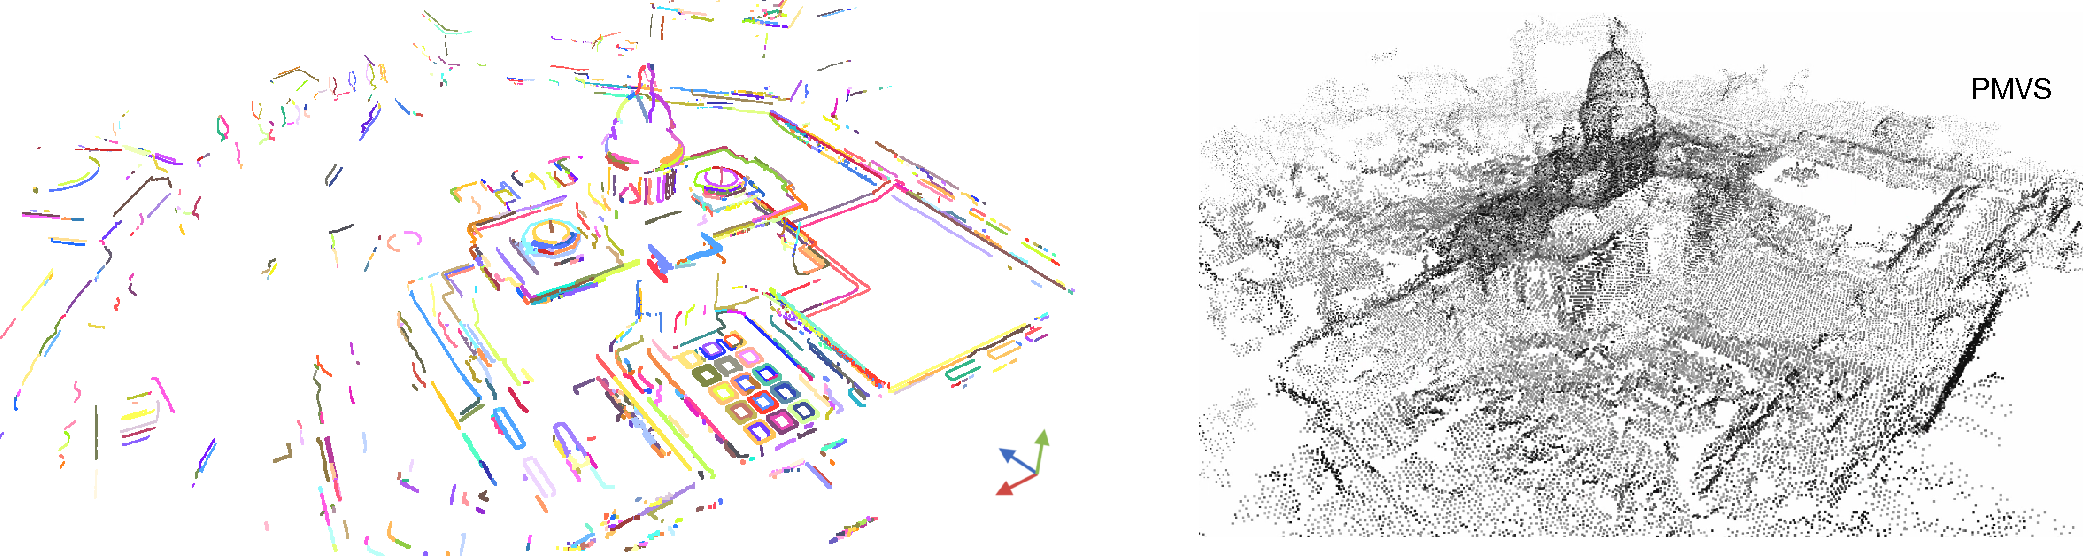
\includegraphics[width=0.95\linewidth]{figs/rec3d-curves-pmvs.pdf}
% 	\label{fig:rec3d}
% 	\caption{A reconstrução usando-se apenas imagens, sem controle de aquisição, 
% 	   como em um vídeo de um smartphone filmado em torno do objeto, fornece uma
% 	   nuvem de pontos, que pode ser
% 	   densificada~\cite{snavely2010bundler,wu2011visualsfm,furukawa2007dense,mve}, ou
% 	   atribuída de
% 	   curvas~\cite{Usumezbas:Fabbri:Kimia:ECCV16,Fabbri:Kimia:IJCV2016,Fabbri:Kimia:CVPR10,Fabbri:Giblin:Kimia:ECCV12}, de forma a preservar a resolução
% 	   em áreas de alto conteúdo informativo. Tais representações estão sendo
% 	   atualmente unificadas na pesquisa da área. Este projeto propõe explorar os
% 	   limites da reconstrução 3D usando-se apenas imagens, no contexto de
% 	   preservação de patrimônio.}
% \end{figure}


Idealizado e criado por Geraldo Simplicio (Nêgo), artista cearense que mora no
local a mais de 30 anos, e que ganhou notoriedade por suas esculturas de barro,
com traços singulares e técnicas únicas. Hoje, trabalha para reconstruir o
Jardim após a tragédia de 2011 na região serrana, onde algumas estruturas foram
destruídas. Portanto, com o consentimento do Nêgo, surgiu a motivação desta
pesquisa: além de explorar métodos de reconstrução, também tem o objetivo de
ajudar a criar sistemas completos para eternizar um patrimônio que é reconhecido
no mundo todo.

A preservação das esculturas do Jardim do Nêgo se mostra um desafio à pesquisa em
recontrução 3D, pois apresentam curvas bem delineadas, que são 
representadas de maneira suavizada e empobrecida por métodos convencionais.
Algumas esculturas apresentam pouca textura, com apenas um leve padrão de musgo.
Seria de grande interesse avaliar o potencial de técnicas atuais de
reconstrução 3D geral que não exigem controle preciso de aquisição, as quais têm seu código fonte
disponível na internet.

\newpage

\section{Objetivos}\label{sec:objetivos}

Pretende-se, ao longo deste projeto, ganhar experiência com técnicas
modernas de reconstrução 3D fotogramétrica, no contexto de uma aplicação
bem-definida de preservação de patrimônio. 
% A entrada do sistema deverá ser um
% conjunto de vídeos realizados por câmeras de baixo custo, ou um conjunto de
% escaneamentos realizados por escaneadores à mão de baixo custo baseados em Kinect.

O objetivo concreto é explorar as tecnologias supracitadas para
desenvolver um esquema de escaneamento de patrimônio usando software aberto, câmeras e
escaneadores de baixo custo, representando o estado da arte em reconstrução 3D sem
restrições de aquisição. Perguntas fundamentais a serem respondidas são: que
nível de detalhe, facilidade e precisão se pode obter usando-se apenas imagens e software
aberto? É possível utilizar escaneadores de baixo custo baseados em Kinect com
melhorias significativas em termos de qualidade, conveniência ou tempo de
processamento?  Quais são as restrições desses sistemas? Seria útil, na prática,
uma reconstrução de curvas para auxiliar na reconstrução de nuvem de pontos e de
superfícies densas? Onde o estado da arte deve ser avançado de forma a permitir
uma solução mais conveniente e completa para a preservação de patrimônio?

O principal objetivo em termos de pesquisa científica será comparar as
diferentes abordagens do estado da arte disponíveis para reconstrução 3D e
explicitar suas limitações práticas.

\section*{Organização deste manuscrito}

Este trabalho foi estruturado da seguinte maneira: previamente, introduzimos métodos baseados em reconstrução a laser, no Capítulo~\ref{cap:laser}, apresentando, de uma maneira mais técnica, o projeto das esculturas de Michelangelo na Seção~\ref{sec:David}, que foi um dos pioneiros na técnica de conservação de acervos culturais. No próximo Capítulo~\ref{cap:kinect}, discutimos o uso do Kinect, da Microsoft, no que tange a calibração do sistema para o uso em tecnologias Structure from Motion. 
Adiante, no Capítulo~\ref{cap:pontosdeinteresse}, abordaremos o tema central do trabalho: técnicas de reconstrução baseadas em fotogrametria, com o emprego de dois softwares, o MVE~\ref{sec:mve} e o VisualSfM~\ref{sec:visualsfm} e seus respectivos funcionamentos. Finalmente, apresentamos experimentos e conclusões do trabalho, bem como sugestoões para implementações e trabalhos futuros.

% O trabalho foi estruturado da seguinte maneira: previamente introduzimos os métodos baseados em pontos de interesse no Capítulo~\ref{sec:pontosdeinteresse}, destacando suas funcionalidades. No Capítulo~\ref{sec:denserecon} discutimos e aprofundamos o  funcionamento de cada algoritmo de reconstrução densa empregados, apresentando e debatendo, comparativamente, pontos à favor e contra; O Capítulo~\ref{sec:kinect} é apresentada a técnica de reconstrução utilizada nos  {\it Kinects}, da Microsoft; Com isso, temos o  Capítulo~\ref{sec:visualsfm}, que é dedicado à ferramenta gráfica utilizada para a obtenção dos resultados (VisualSfM) dos algoritmos de reconstrução densa utilizados. Finalmente, apresentamos os resultados e conclusões do trabalho, bem como sugestões para implementações e trabalhos futuros.
%Este trabalho está organizado da seguinte forma: discutimos as técnicas de
%extração de curva sem aprendizagem de máquina supervisionada no
%Capítulo~\ref{sec:cfrag:extraction}. No Capítulo~\ref{sec:learning:chapter},
%discutimos maneiras pelas quais essas técnicas podem ser melhoradas
%usando dados de treinamento anotados por humanos como entrada para uma
%aprendizagem de máquina geométrica de topologia e semântica de fragmentos de
%curva. A maior parte deste material é
%de~\cite{Guo:etal:CVPR14,Guo:etal:PAMI2017:submitted,Tamrakar:PHD:2008}, com esclarecimentos
%substanciais e comentários sobre as questões relativas aos nossos objetivos
%específicos. No Capítulo~\ref{sec:generic:datasets}, apresentamos o processo de
%captura de dados confiáveis (\emph{ground-truth}), comparando os conjuntos de dados anteriores com o problema proposto
%neste trabalho para a água. Nos capítulos restantes, apresentamos e discutimos
%nossos resultados para vários vídeos em tanques de água. Partes deste trabalho
%foram apresentadas em~\cite{Fabbri:WaterWaves2016,Fabbri:WaterWaves2017,Souza:Fabbri:WaterWaves2017}.

%======================================================================================

\section{Laser}\label{sec:laser}

A técnica de reconstrução baseada em laser é conhecida desde o século passado, pois oferecem uma alta qualidade geométrica de dados, os resultados são em tempo real e requer pouco tempo de captura de dados. 

Existem alguns tipos de reconstruções empregando lasers, baseados em volume (ressonância, tomografia, por exemplo \ref{fig:laservolume} ou em superfície (estereoscopia, {\it time of flight}, luz estruturada) . Neste caso, abordaremos o projeto de escaneamento da escultura de Michelangelo, David, que utiliza escaners baseados em superfícies, mais especificamente, utilizando luz estruturada.

\begin{figure}[!h]
	\centering
	%   \includegraphics[width=1.0\linewidth]{figs/3d-curve-sketch/system-diagram.eps}
	\includegraphics[width=1\linewidth]{figs/tomografia.png}
	\caption{%
	Exemplo de reconstrução à laser utilizando o método baseado em volume.
	%\cite{Cui:Theobalt:etal:PAMI2013,Pajdla:etal:ICCV2011}.
	}\label{fig:laservolume}
\end{figure}

Este projeto tem como motivação avançar a tecnologia de digitalização 3D e criar um acervo digital sobre alguns dos principais artefatos culturais. Foi utilizada uma tecnologia chamada de {\it rangefinder}, com uma equipe de mais de 30 professores, funcionários e estudantes da Universidade de Stanford desenvolveram algoritmos para combinar imagens de múltiplas gamas e cores, passaram os anos de 1998 e 1999 na Itália escaneando esclturas de Michelangelo. 

Pipeline:

O principal componente de {\it hardware} do sistema é um escaner de triangulação à laser, que é composto por 4 eixos motorizados, utiliza um laser, uma câmera de alcance, uma câmera de cores e uma luz branca, isso tudo acrescido de estruturas para estátuas grandes. O objetivo de um escaner deste porte era capturar marcas menores que um milímetro, das ferramentas utilizadas por Michelangelo em suas esculturas. 
Para isso foram testadas diversas resoluções, na qual foi decidido um espaçamento Y (ao longo da faixa do laser) de 1/4 mm e uma resolução Z (profundidade) de pelo menos duas vezes este valor. O que resultou em uma visualização de 14 cm de largura (ao longo da faixa do laser) por 14 cm de profundidade. Caso esta resolução fosse menor, as marcas de cinzelão ficariam borradas e se fosse maior, o conjunto de dados produzido seria gigantesco.
Felizmente, a maioria das estátuas feitas por Michelangelo foram esculpidas com um mármore encontrado em Carrara Statuario, uma pedra altamente uniforme, não direcional e constituída de grãos finos. Além disso, com exceção da "Noite", as esculturas não são polidas e cobertas por terra, o que aumenta a dispersão superficial e reduz a abaixo da superfície.
Neste contexto, a dispersão abaixo da superfície causa alguns problemas: não se pode assumir que a superfície é Lambertiana ideal (%CITAR LAMBERTIANO AQUI%
), mudou a forma com que a renderização dos modelos seriam feitos e diminuiu a qualidade de disposição de dados 


% Depois de testar várias resoluções, decidimos um espaçamento de amostra Y (ao longo da faixa laser) de 1/4 mm e uma resolução Z (profundidade) pelo menos duas vezes esta multa 1. Isso nos deu uma visão de 14 cm de largura (ao longo da faixa a laser ) por 14 cm de profundidade. Em retrospectiva, ficamos satisfeitos com a resolução que escolhemos; Qualquer coisa menor teria significativamente borrado as marcas de cinzelão de Michelangelo, e qualquer coisa maior teria tornado os nossos conjuntos de dados não gerenciáveis.

%FIGURA DAS FERRAMENTAS AQUI%


% The main hardware component of our system was a laser triangulation
% scanner and motorized gantry customized for digitizing
% large statues. Our requirements for this scanner were demanding;
% we wanted to capture chisel marks smaller than a millimeter, we
% wanted to capture them from a safe distance, and we wanted to
% reach the top of Michelangelo’s David, which is 23 feet tall on its
% pedestal. In the sections that follow, we describe the range and
% color acquisition systems of this scanner, its supporting mechanical
% gantry, and our procedure for calibrating it.

% O principal componente de hardware do nosso sistema foi um scanner de triangulação a laser e um pórtico motorizado personalizado para digitalizar grandes estátuas. Nossos requisitos para este scanner eram exigentes; queríamos capturar marcas de cinzelão menores do que um milímetro, queríamos capturá-las a uma distância segura, e queríamos chegar ao topo do David de Michelangelo, que tem 23 pés de altura no pedestal. Nas seções que se seguem, descrevemos os sistemas de aquisição de alcance e cor deste scanner, seu pórtico mecânico de suporte e nosso procedimento para calibrá-lo.

Primeiramente faz-se o escaneamento da geometria da escultura:
\begin{itemize}
\item{Alinhamento manual}
\item{ICP -- {\it Iterative Closest Point} para uma câmera existente} %CITAR ICP AQUI%
\item{ICP automático para todos os pares sobrepostos}
\item{Relaxação global para espalhar o erro}
\item{Reunir utilizando métodos volumétricos}
\end{itemize}


Após isso, ocorre o escaneamento e processamento das cores da escultura:

\begin{itemize}
\item{Compensação da iluminação do ambiente}
\item{Descarte de pixels com sombra ou especulares}
\item{Mapeia-se os vértices (uma cor por vértice)}
\item{Correção da irradiância e reflectância difusa}
\end{itemize}

Limitações:
\begin{ìtemize}
\item{Inter-reflexões são ignoradas}
\item{Dispersões subterrâneas são ignoradas}
\item{Tratamento difuso com Lambertiano} %CITAR TREATED DIFFUSED AS LAMBERTIAN%
\item{Usa superfícies normais agregadas}

\end{itemize}

O projeto não teve mais nenhum avanço desde o verão de 2004, por falta de financiamento. Como resultado, modelos de alta qualidade só existem do David na resolução de 1,0 mm (56 milhões de triângulos) e São Mateus a 0,25 mm (372 milhões de triângulos). Um modelo também existe para o Atlas em 0,25 mm (aproximadamente 500 milhões de triângulos), mas contém erros de alinhamento. Após 6 anos de trabalho estudantil remunerado e voluntário, existem modelos para cada um dos 1.186 fragmentos. Esses modelos, que totalizam quase 8 bilhões de polígonos, se encontram no próprio site da Universidade de Stanford %CITAR AQUI$. 

Também foram disponibilizadas algumas métricas sobre este projeto \ref{tab:metricasDavid}.

\begin{table}
\caption{Algumas métricas do projeto}
\label{tab:metricasDavid}
\begin{tabular}{|l|l|}
\hline
Números de objetos escaneados          & 10 estátuas + 2 edificações + 1,163 fragmentos de mapa  \\ \hline
Menor e maior objetos escaneados       & 1 polegada (fragmentos de mapa) e 23 pés (David)         \\ \hline
Resolução espacial dos dados                & 0.29mm para geometria, 0.125mm para cor              \\ \hline
Complexidade do maior conjunto de dados             & 2 bilhões de polígonos + 7,000 imagens (David)\\ \hline
Tamanho do maior conjunto de dados                    & 32 {\it gigabytes} (David)                  \\ \hline
Quantia total de dados capturados              & 250 {\it gigabytes}                                 \\ \hline
Tamanho do maior escaner                    & 24 pés de altura, 1800 libras de peso                  \\ \hline
Peso total do equipamento levado para a Itália & 4 toneladas                                              \\ \hline
Número de pessoas envolvidas                  & 32 (sem incluir subcontratantes e colaboradores) \\ \hline
Tempo médio para escaneamento              & 1 semana (exceto o David, que levou 1 mês)       \\ \hline
Tempo total de escaneamento                 & 5,000 horas de trabalho                                   \\ \hline
Total de tempo para processamento de dados          & 4,000 horas de trabalho (até agora)                            \\ \hline
Custo do projeto                          & \$2,000,000                                         \\ \hline
\end{tabular}
\end{table}
%COLOCAR FOTOS DAVID%
Porém, devido ao seu alto custo com equipamentos, com {\it softwares} e sem falar na necessidade de estações robustas para armazenamento dos dados e para esacaneamento de patrimônios, outras técnicas foram emergindo com o passar dos anos, como a fotogrametria, que será abordada mais tarde neste documento.
\chapter{Kinect}\label{sec:kinect}
%======================================================================================
Um componente criado pela Microsoft para fins recreativos (como no XBox, por exemplo), virou uma das mais conhecidas ferramentas de reconstrução 3D no cenário atual. Sua primeira versão (Kinect V1) utiliza uma técnica similar à empregada no projeto da Universidade de Stanford, com luz estruturada, porém, diferentemente dos escaners à laser, o Kinect tem um custo monetário baixo e é acessível a todo público em geral (desde entusiastas, amadores até profissionais da área). 

O Kinect V2 utiliza uma projeção de fótons [...] e por isso ele já não é tão utilizado na área de reconstrução 3D como o V1. 

O V1 é composto por 2 câmeras: uma RGB e outra de profundidade e por um projetor IR ({\it infra-red}) de padrões. E funciona da seguinte maneira: o projetor IR de padrões lança uma matriz que é conhecida pelo Kinect, a partir disso, qualquer deformação deste padrão é captada pelas câmeras, o que identifica se um objeto está no alcance dos sensores ou não. A resposta, é composta por 3 {\it outputs}: uma imagem IR,  uma RGB e a profundidade (inversa) da imagem.

%IMAGEM KINECT%

Sua principal saída da imagem do Kinect é correspondente à profundidade da cena. Em vez de providenciar uma profundidade {\it Z}, ele retorna uma profundidade inversa, {\it D}.
A profundidade da imagem é construída a partir da triangulação da imagem IR com o projetor e, consequentemente, "carregada" pela imagem IR.

%IMAGEM PROFUNDIDADE KINECT%
 
Foram realizados alguns experimentos associando fotogrametria com o Kinect V1. Primeiramente, foi executado uma calibração do Kinect para este tipo de reconstrução, onde a partir de experimentos, o sistema foi modelado como \ref{eq:kinectCalibracao}.

\begin{equation}
q(z) = 2.73 z^2 + 0.74 z − 0.58 [mm]
\label{eq:kinectCalibracao}
\end{equation}

Onde "z" é a profundidade em metros, e "q" a quantização.

O modelo geométrico do kinect foi criado com um sistema multi-view considerando o RGB, IR e a profundidade
\begin{equation}
\begin{bmatrix}u \\v \\ 1 \end{bmatrix} = K \begin{bmatrix}s \\t \\ 1 \end{bmatrix}
\end{equation}

Entretanto, uma desvantagem que diminui a aplicabilidade do Kinect é que ele foi projetado para funcionar bem em espaços fechados, com detecção de formas humanas e movimentações. Ou seja, numa aplicação {\it in situ} ele já não funcionaria muito bem, pois além de não conseguir projetar os detalhes em alta definição de uma escultura, ele necessita de uma fonte de energia externa, o que dificulta a acessibilidade do mesmo e como gera uma reconstrução em tempo real (não tem uma forma de salvar em {\it cache} ou internamente), ele precisa estar ligado a um computador para fazer o escaneamento.
\chapter{Pontos de Interesse}\label{sec:pontosdeinteresse}
%======================================================================================
%
A reconstrução 3D pelo método da estrutura do movimento, ou {\it Structure from Motion} ({\it SfM}). Tem como base a utilização de pontos de interesse
({\it features}), que são pontos ou áreas em comum entre as imagens usadas na reconstrução. Para encontrar estes pontos, diferentes algoritmos são empregados.

\section { SIFT -- {\it Scale Invariant Feature Transform}}

Primeiramente, utiliza-se o SIFT (algoritmo de detecção de pontos de interesse, invariante à escala e à transformações, como rotação, translação e iluminação da imagem, por exemplo).
O algoritmo pode ser dividido em cinco etapas, das quais:

\begin{itemize}
	\item{Deteccão de espaço-escala extremos -- {\it Scale-space Extrema Detection}}
	\item{Localização de pontos-chaves -- {\it Keypoint Localization}}
	\item{Atribuição de orientação -- {\it Orientation Assignment}}
	\item{Descritor de pontos-chaves -- {\it Keypoint Descriptor}}
	\item{Combinação de pontos-chaves -- {\it Keypoint Matching}}
\end{itemize}


\subsection{Detecção de espaço-escala extremos}

% From the image above, it is obvious that we can't use the same window to detect keypoints with different scale. It is OK with small corner. But to detect larger corners we need larger windows. For this, scale-space filtering is used. In it, Laplacian of Gaussian is found for the image with various σ values. LoG acts as a blob detector which detects blobs in various sizes due to change in σ. In short, σ acts as a scaling parameter. For eg, in the above image, gaussian kernel with low σ gives high value for small corner while guassian kernel with high σ fits well for larger corner. So, we can find the local maxima across the scale and space which gives us a list of (x,y,σ) values which means there is a potential keypoint at (x,y) at σ scale.

Em casos com cantos pequenos, a detecção funciona bem. Porém, raramente utilizaremos a mesma janela para detectar pontos-chaves em imagens com diferentes escalas, pois utilizamos imagens grandes e, consequentemente, cantos grandes. Para isso, precisamos de janelas grandes também. 

Para resolver este problema, o filtro de escala-espaço é usado: o Laplaciano de Gaussiano ({\it Laplacian of Gaussian} --  LoG). O LoG atua como um detector de particulas em diferentes tamanhos $\sigma$. (Onde $\sigma$ é o parâmetro de escala). Por exemplo, o núcleo gaussiano com $\sigma$ baixo, tem como resposta um alto valor para um canto pequeno. Enquanto um núcleo gaussiano com alto $\sigma$, se encaixa bem para um canto maior. Com esta lógica, podemos encontrar um máximo local através da escala e o espaço, o que nos fornece uma lista de $(x,y \sigma)$, o que significa que existe um ponto-chave em potencial, com o par $(x,y)$ na escala $\sigma$.

% \begin{equation}
% LoG(x,y) = - \frac{1}{\pi \sigma ^4 }\left [ 1 - \frac{x^2+y^2}{2 \sigma ^2} \right ]e^{- \frac{x^2+y^2}{2 \sigma ^2}} 
% \end{equation}

Porém, como o LoG é um pouco custoso, computacionalmente. O SIFT utiliza um algoritmo aproximado do LoG, o DoG (Diferença de Gaussianos -- {\it Difference of Gaussians}). O DoG é a diferença de um filtro Gaussiano de uma imagem, com dois valores diferentes de escala $\sigma$. 

Uma aplicação prática do filtro DoG é a sequência de imagens a seguir:

\begin{figure} [!h]
	\centering
	\includegraphics[width=0.45\linewidth]{figs/lena.jpg}(a)
	\includegraphics[width=0.45\linewidth]{figs/lenaSigma1.png}(b)
	\includegraphics[width=0.45\linewidth]{figs/lenaSigma2.png}(c)
 	\includegraphics[width=0.45\linewidth]{figs/lenaDoG.png} (d)
	\caption{%
	É aplicado um filtro gaussiano na imagem original (a), com $\sigma$ = 1, tendo como resultado a imagem (b).
	Um outro filtro gaussiano é usado, porém, neste caso, o $\sigma$ = 2 (c). Após isso, subtrai-se (b) de (c), obtendo 
	o filtro DoG (d).
	}\label{fig:lenadog}
\end{figure}

Uma vez que o DoG é aplicado, as iamgens são utilizadas com o espaço e escala extremos. Por exemplo, na imagem \ref{fig:extrema}, um pixel é comparado com seus 8 vizinhos, assim como comparado com os 9 pixels na próxima escala e os 9 pixels na escala anterior. Se esse pixel é um local extremo, ele é um ponto-chave em potencial. Isto é, este ponto-chave é melhor representado nesta escala.

\begin{figure}
	\centering
	\includegraphics[width=0.45\linewidth]{figs/sift_local_extrema.jpg}
	\caption{%
	Exemplo de funcionamento de deteccão de espaço-escala extrema
	}\label{fig:extrema}
\end{figure}

No caso, as funções ficariam da seguinte forma: 

\begin{equation}
\label{eq:gaussiano}
	g_\sigma(x) = \frac{1}{2 \pi \sigma ^2} e^{-\frac{1}{2} \frac{x^T x}{\sigma ^2}}
\end{equation}

\begin{equation}
\label{eq:gaussianScaleSpace}
	I_\sigma = g_\sigma * I, \sigma >= 0
\end{equation}

\begin{equation}
\label{eq:LoG}
	\triangledown^2	g_\sigma(x)
\end{equation}

\begin{equation}
\label{eq:DoG}
	DoG_\sigma(o,s) = I_\sigma(o,s+1) - I_\sigma(o,s)
\end{equation}


Onde \ref{eq:gaussiano} é a função padrão do operador gaussiano (núcleo), a equação \ref{eq:LoG} é o operador LoG,  \ref{eq:DoG} é o operador DoG e $\triangledown^2$ é o operador Laplaciano.

\subsection{Localização de pontos-chaves}

A localização dos pontos extremos pode cair em um extremo local e não global. Logo, após a utilização do DoG e com os pontos-chaves em potencial localizados, eles precisam ser refinados para melhorar o resultado. Para isso, são utilizadas Séries de Taylor na escala e no espaço, e, se a intensidade nesse extremo é menor que o valor limite, este é rejeitado.
%TODO: Ver isso 
Os {\it frames} do SIFT (pontos-chaves) são extraídos baseados nos extremos locais (picos) a partir do DoG. Numericamente, extremos locais são elementos que possuem um menor (ou maior) valor em uma vizinhança em um espaço 3x3x3 (em escala e espaço).
Depois de extraídos, estes pontos são interpolados quadraticamente (este passo é muito importante, especialmente nas escalas de menor resolução, para ter uma localização precisa do ponto-chave na resolução completa). Finalmente, eles são filtrados para eliminar respostas de baixo contraste ou respostas próximas as bordas.

%Eliminating low contrast responses

Picos que são pequenos, na maior parte das vezes são gerados a partir de ruídos e necessitam ser descartados também. Isso é feito com uma comparação de valor absoluto do DoG no pico com o valor do pico limite e é descartado caso este valor é menor que o limite.


%Eliminating edge responses 

Para eliminar respostas em bordas, normalmente os picos mais rasos ou horizontais, são gerados por bordas e não possuem características estáveis, portanto estes picos precisam ser removidos. Para isso, dado um pico (x, y, $\sigma$), o algoritmo avalia a matriz Hessiana (x,y) do DoG na escala $\sigma$. Então é computado um valor para esta equação (\ref{eq:hessianaDoG}):

\begin{equation}
	v = \frac{( T_r \ D(x,y,\sigma))^2}{Det \ D(x,y,\sigma)}
	\label{eq:hessianaDoG}
\end{equation}
Onde, $T_r$ é o traço, ou seja, $T_r(H) = D_{xx} + D_{yy}$ e a matriz $D$ é do tipo
\[D = \begin{bmatrix}
	\frac{\partial ^2 DoG}{\partial x^2} & \frac{\partial ^2 DoG}{\partial x \partial y} \\ 
	\frac{\partial ^2 DoG}{\partial x \partial y} & \frac{\partial ^2 DoG}{\partial y^2} 
\end{bmatrix}
\]

No caso, v possui um valor mínimo (igual a 4) quando os autovalores da Jacobiana são iguais (pico curvado) e aumentam à medida que um dos autovalores aumenta e os outros permanecem baixos. Os picos são retidos se $v  < \frac{(t_e+1)(t_e+1)}{t_e}$ , onde $t_e$ é o limite da borda. 

\subsection{Atribuição de orientação}

Agora, uma orientação é atribuída a cada ponto-chave para obter a invariância à rotação da imagem. 
Uma vizinhança é obtida, dependente da escala, do gradiente da magnitude \ref{eq:magnitudeSIFT} e da direção \ref{eq:direcaoSIFT} (usando diferenças finitas), ao redor da localização do ponto-chave. 

\begin{equation}
	m(x,y) = \sqrt{(L(x+1,y)-L(x-1,y))^2 + (L(x,y+1)-L(x,y-1)^2)}
	\label{eq:magnitudeSIFT}
\end{equation}

\begin{equation}
	\theta = tan^{-1} \left( \frac{(L(x,y+1)-L(x,y-1)}{(L(x+1,y)-L(x-1,y)}\right)
	\label{eq:direcaoSIFT}
\end{equation}

Então, um histograma de 36 orientações ({\it bins}) cobrindo 360 graus é criado. Onde ele é ponderado pelo gradiente da magnitude e por uma janela Gaussiana circular onde $\sigma$ vale $1.5$ em relação à escala do ponto-chave \ref{fig:histogramaOrientado}.

\begin{figure} [!h]
	\centering
	\includegraphics[width=0.45\linewidth]{figs/histogramaOrientado.png}
	\caption{%
	Exemplo do resultado obtido do histograma orientado
	}\label{fig:histogramaOrientado}
\end{figure}

O ponto mais do histograma é obtido e qualquer pico acima de 80\% é considerado no cálculo da orientação. 
Pontos-chaves são criados com a mesma localização e escala, mas em diferentes direções, o que contribui para a establidade da correspondência.

\subsection{Descritor de pontos-chaves}

Com os pontos-chaves criados a partir do histograma orientado, cria-se agora o descritor de pontos-chaves.

Uma vizinhança 16x16 ao redor do ponto-chave é escolhida e esta mesma vizinhaça é dividida em 16 sub-blocos 4x4. Para cada bloco, um histograma orientado com 8 {\it bin} é criado. Logo, temos 128 valores válidos de {\it bin}. Esses valores são representados em forma de vetor para expressar o descritor de pontos-chaves \ref{fig:descritorKeypoint}. 

Além disso, são tomadas algumas medidas para deixar o descritor mais robusto,como, por exemplo, invariante à luminosidade, rotação, etc.

\begin{figure} [!h]
	\centering
	\includegraphics[width=0.45\linewidth]{figs/descritorKeypoint.png}
	\caption{%
	Exemplo de um descritor de pontos-chaves, com uma matriz 2x2 e uma região 8x8
	}\label{fig:descritorKeypoint}
\end{figure}

\subsection{Combinação de pontos-chaves}

Pontos-chaves entre duas imagens são combinados a partir da identificação da vizinhança mais próxima. Mas, em alguns casos, a segunda combinação mais próxima pode ser parecida com a primeira. Isso se dá por ruídos presentes nas imagens ou algo assim. 

Nesse caso, a razão da distância mais próxima para a segunda distância mais próxima é utilizada. Se essa razão for maior que 0.8, essa combinação é descartada.
Esse método elimina cerca de 90\% de combinações falsas, enquanto descarta apenas cerca de 5\% de combinações corretas.

\section {Triangulação -- {\it Full pairwise image matching}}

Com os pontos de interesse ({\it features}) extraídos, podemos agora fazer a triangulação entre os pontos das imagens.

A triangulação nada mais é que uma estimativa de um ponto em 3 dimensões, dado pelo menos duas câmeras conhecidas, onde, cada câmera com a projeção do {\it feature} correspondente àquele ponto 3D \ref{fig:triangulacao}.

\begin{figure} [!h]
	\centering
	\includegraphics[width=0.45\linewidth]{figs/triangulacao.png}
	\caption{%
	Uma triangulação utilizando um ponto qualquer, $X_j$. Onde cada câmera $C_1, C_2, C_3$ possui um {\it feature} correspondente a cada uma delas, respectivamente, $X_{1j}, X_{2j}, X_{3j}$.
	}\label{fig:triangulacao}
\end{figure}

Infelizmente, não é tão simples assim. Existem muitos fatores que contribuem para aumentar a dificuldade da triangulação: ruídos, posição das câmeras, o feixe das projeções não se encontram no mesmo ponto 3D, não se tem informação da projeções nas câmeras, etc. Entretanto, existem diversos algoritmos para resolução de cada um dos problemas enfretados.

Como o foco deste manuscrito está no {\it software} de reconstrução VisualSfM, atentamos apenas ao algoritmo utilizado pelo mesmo. Neste caso, ele utiliza um algoritmo chamado {\it Bundle Adjustment}. 

Este algoritmo é utilizado para minimizar o erro geométrico proveniente da reprojeção da triangulação \ref{fig:triangulacaoErro}. Dentro dele, existe a técnica de resolução de problemas não-lineares chamada Levenberg-Marquardt.

\begin{figure} [!h]
	\centering
	\includegraphics[width=0.45\linewidth]{figs/triangulacaoErro.png}
	\caption{%
	Erro proveniente da reprojeção, onde os pontos $x$ e $x'$ estão mais próximos das medidas reais da imagem. 
	}\label{fig:triangulacaoErro}
\end{figure}


\chapter{VisualSfM}\label{sec:visualsfm}
%======================================================================================
%
\section*{Introdução}

VisualSfM é um {\it software} baseado em fotogrametria que faz todo o processo de reconstrução 3D de um objeto e que pode usá-lo por linha de comando ou então pela interface gráfica, que é ótima, por sinal. É altamente customizável, podendo utilizar o CUDA da NVIDIA ou OpenGL, especificar a lista de pares para correspondência de imagens, usar detectores de {\it features} próprios, velocidade da detecção de {\it features}, da reconstrução densa, dentre outros parâmetros. Ou seja, é um {\it software} robusto, que pode ser usado em Linux, Windows ou até mesmo Mac.

\section*{Procedimento}

Sua linha de reconstrução é parecida com o MVE \ref{sec:mve}, porém é mais intuitiva. Em sua interface, possui um Log de mensagens e erros que por ventura venham a acontecer e na parte de cima, alguns botões \ref{fig:pipelineVisualSfM}

\begin{figure}[!h]
	\centering

	\includegraphics[width=1\linewidth]{figs/pipelinevisualsfm.png}
	\caption{%
	Botões na parte superior da interface gráfica, este seria o {\it pipeline} padrão de funcionamento do {\it software}.
	}\label{fig:pipelineVisualSfM}
\end{figure}

Como demonstrado na imagem \ref{fig:pipelineVisualSfM}, o funcionamento seria da seguinte forma:

\begin{itemize}
\item \textbf{1 - Adicionar algumas imagens.} Este é o primeiro passo, para começar uma reconstrução, primeiro adiciona-se imagens ao {\it software}, pode ser uma única foto, um conjunto de fotos, incrementar o conjunto já existente ou então abrir um arquivo de extensão .nvm, que é interpretado como uma reconstrução esparsa previamente feita.

\item \textbf{2 - Correspondência de imagens.} Agora, o {\it software} roda o algoritmo SIFT, realizando todas as correspondências entre os {\it features}.

\item \textbf{3 - Reconstrução esparsa.} Neste passo, o VisualSfM roda o algoritmo de reconstrução esparsa (PBA). %LEMBRAR QUAL É O ALGORITMO!!% 

esparsa em todos os {\it features} descobertos no passo passado.

\item \textbf{4 - Reconstrução densa.} Finalmente, acaba a reconstrução rodando o algoritmo CMVS/PMVS-2 embutido no próprio VisualSfM de reconstrução densa.
\end{itemize}

PBA -- {\it Parallel Banding Algorithm}

O PBA é um algoritmo implementado em GPU (Graphic Processor Unit) para computar a Distância de Transformação Euclidiana (EDT -- Euclidean Distance Transform) para uma imagem binária em 2D ou em dimensões superiores. Particionando a imagem em pequenas bandas para processar e posteriormente, juntando-as simultaneamente, o PBA calcula o EDT exato com ótimo trabalho linear total, alto nível de paralelismo e um bom padrão de acesso à memória. Este algoritmo foi um dos precursores ao tentar explorar o máximo desempenho da GPU no cálculo da EDT exata. 


% O PBA é divido em 3 fases:

% \begin{itemize}
% \item Band Sweeping
% \item Hierarchical Merging
% \item Block coloring
% \end{itemize}

% Band Sweeping

% In this phase, for each row, we want to compute the 1D Voronoi
% diagram using only those sites in the same row. A trivial approach
% would be to use a two-pass sweeping (left to right and then right to
% left sweeping), similar to SKW [Schneider et al. 2009]. This, however,
% restricts the parallelism to only one thread per row, potentially
% under-utilizing the GPU. One could also use a 1D JFA [Rong and
% Tan 2007] with better utilization of the GPU at the cost of higher
% total work. Another possibility would be to use a method similar
% to the work efficient parallel prefix sum [Harris et al. 2007]. This
% approach is too complicated as compared to our following simple,
% yet work and time efficient approach.
% Our approach extends the na¨ıve two-pass sweeping approach, with
% the introduction of bands to effectively increase the level of parallelism.
% First, we divide the input image into m1 vertical bands
% of equal size, and use one thread to handle one row in each band,
% performing the left-right sweeps. Next, for one site to propagate
% its information to a different band (on the same row), it has to be
% the closest site to the first or the last pixel of its band. As such, to
% combine the result of different bands into the needed answer, we
% first propagate the information among the first and the last pixels
% of all bands using a parallel prefix approach on these 2m1 pixels.
% With this, the first and the last pixel of each band have the correct
% information, whereas other pixels inside a band can then obtain the
% correct closest sites by updating (if needed) their current information
% with that of the first and the last pixel of their band. This can
% be done in parallel in constant time using N threads.

% Hierarchical Merging




%FALAR SOBRE O ALGORITMO DE RECONSTRUCAO DENSA == PMVS-2/CMVS%

Algoritmo de reconstrução densa - CMVS/PMVS-2 (Clustering Views for Multi-view Stereo)

%Um dos algoritmos mais utilizados Furukawa o CMVS que possui o PMVS-2 (Patch-based Multi-view Stereo versão 2) implementado dentro dele. O PMVS-2 é uma abordagem automatizada para reconstruções densas de superfícies, baseada em combinações de features de imagens múltiplas e técnicas de correspondência baseadas em áreas, com imagens calibradas.
%Ele utiliza conjuntos de imagens e parâmetros de câmera, então reconstrói a estrutura 3D de um objeto, ou a cena visível nas imagens. Um ponto positivo deste {\it software} é que ele só reconstrói estruturas rígidas, ou seja, ele ignora automaticamente objetos não rígidos como pessoas na frente de uma construção ou escultura, por exemplo. A saída do {\it software} é um conjunto orientado de pontos ao invés de um modelo poligonal (ou malha), onde tanto a coordenada 3D quanto a superfície normal são estimados em cada ponto orientado.
%
Muitos algoritmos Multi-view Stereo (MVS) não escalam tão bem com um grande número de imagens de entrada ou em uma alta resolução, pois necessitam de muita memória e recursos computacionais. A palavra-chave do CMVS é escalabilidade, pois seu propósito é utilizar imagens provenientes de sites na internet, em diferentes resoluções, como o Flickr.com.  
O CMVS usa a saída do Structure from Motion -- SfM (mais especificamente a saída do passo anterior, do PBA) e utiliza como entrada. Após isso, decompõe as imagens de entrada como um conjunto de {\it clusters} de imagens com tamanhos gerenciáveis. O MVS pode ser usado para processar cada {\it cluster} de forma independente e em paralelo, onde a união das reconstruções de todos os {\it clusters} não deve perder detalhes que poderiam ser obtidos através do conjunto de imagens.

A formulação dos {\it clusters} é projetada para satisfazer três restrições: (1) as imagens redundantes são excluídas dos {\it clusters} (compacidade), (2) cada {\it cluster} é pequeno o suficiente para uma reconstrução MVS (restrição de tamanho) e (3) as reconstruções MVS destes {\it clusters} resultam em uma perda mínima de conteúdo e detalhes em comparação com o que pode ser obtido através do processamento do conjunto completo de imagens (cobertura).
A compacidade é importante para a eficiência computacional, mas também para melhorar precisão, pois as coleções de fotos da Internet geralmente contêm centenas ou milhares de fotos adquiridas de quase mesmo ponto de vista, ou seja, um conjunto composto inteiramente informações duplicadas.

Em outras palavras, a sobreposição de {\it clusters} é definida por:

\begin{itemize}
\item Minimizar $\sum_{k} |C_k|$ (compacidade)
\item $\forall k |C_k| \le \alpha$, onde $\alpha$ é determinado por recursos computacionais, principalmente por limitações de memória. (tamanho)
\item $\forall i \frac{{# pontos cobertos em I_i}}{{# pontos em I_i}} \ge \delta$, onde $\delta$ é uma constante de proporção de pontos cobertos. (cobertura)
\end{itemize}



Este algoritmo, pode ser separado da seguinte forma:

\begin{itemize}
\item Filtro SFM -- agrupamento de pontos SFM
\item Seleção de imagens -- remove imagens reduntantes
\item Divisão de {\it cluster} -- reforça a restrição de tamanho
\item Adição de imagens -- reforça a cobertura
\end{itemize}


\subsection{Filtro SFM}

A obtenção de medidas precisas de visibilidade de pontos é fundamental para o sucesso do nosso procedimento de visualização baseado em {\it clusters}. Os recursos da imagem não detectados ou incomparáveis ​​levam a erros nas estimativas de visibilidade do ponto $V_j$ (geralmente na forma de imagens que estão faltando). Obtemos estimativas de visibilidade mais confiáveis ​​ao agregar dados da visibilidade em uma vizinhança local, e mesclando pontos nessa vizinhança. A posição do ponto mesclado é a média de seus vizinhos, enquanto a visibilidade se torna a união. Este passo também reduz significativamente o número de pontos SFM e melhora o tempo de execução das três etapas restantes. Especificamente, a partir de um conjunto de pontos SFM, selecionamos aleatoriamente um ponto, combinamos com seus vizinhos, emitimos o ponto mesclado e removemos o ponto e seus vizinhos do conjunto de entrada. Repetimos o procedimento até o conjunto de entrada estar vazio. O conjunto de pontos mesclados torna-se o novo conjunto de pontos, que, com algum abuso de notação, também é denotado como ${P_j}^2$. %Figura 4%


\subsection{Seleção de imagens}

Começando com o conjunto completo de imagens, cada imagem é testada e removida se a restrição de cobertura ainda for realizada após a remoção. O teste de remoção é realizado para todas as imagens enumeradas em ordem crescente de resolução de imagem (# de pixels), de modo que as imagens de baixa resolução sejam removidas primeiro. Observe que as imagens são descartadas permanentemente nesta etapa para acelerar as seguintes etapas principais de otimização.

\subsection{Divisão de {\it cluster}}

Em seguida, é aplicada a restrição de tamanho dividindo os {\it clusters}, ignorando a cobertura. Mais especificamente, um {\it cluster} de imagens é dividido em componentes menores caso viole a restrição de tamanho. A divisão de um {\it cluster} é realizada pelo algoritmo {\it Normalized-Cuts} %CITAR#
[23] em um gráfico de visibilidade, onde os nós são imagens. O peso dA borda entre um par de imagens ($I_l, I_m$) mede o quanto a $I_l$ e $I_m$ contribuem, juntos,  para a reconstrução MVS em pontos SFM relevantes: 

$e_{lm} = \sum_{P_j \in \Theta ^{lm} \frac{f(Pj,{Il, Im})}{f(Pj, Vj )}$, onde $\Theta ^{lm}$ denota um conjunto de pontos SFM visíveis em $L_l$ e $I_m$. Intuitivamente, as imagens com alta contribuição no MVS têm pesos altos entre eles e são menos propensos a serem cortados. A divisão de um {\it cluster} se repete até que a restrição de tamanho seja satisfeita para todos os {\it clusters}.

\subsection{Adição de imagens}

A restrição de cobertura pode ter sido violada na etapa anterior, e agora são adicionadas imagens a cada {\it cluster} para cobrir mais pontos SFM e restabelecer a cobertura. Nesta etapa, primeiro é construída uma lista de ações possíveis, onde cada ação mede a eficácia de adicionar uma imagem a um {\it cluster} para aumentar a cobertura. Para cada ponto SFM que está descoberto, $P_j$, deixe $C_k = argmax_{Cl} f(Pj, Cl)$ ser o {\it cluster} com a máxima precisão de reconstrução. 
Então, para $P_j$, é criada uma ação ${(I \rightarrow C_k), g}$ que adiciona a imagem $I (\in V_j, \not\in C_k)$ a $C_k$, onde $g$ mede a eficácia. Só são consideradas ações que adicionam imagens ao $C_k$ em vez de cada {\it cluster} que poderia cobrir $P_j$, para eficiência computacional. Uma vez que as ações com a mesma imagem e com o mesmo {\it cluster} são geradas a partir de vários pontos SFM, ocorre uma mescla dessas ações ao resumir a eficácia medida $g$. As ações na lista são classificadas em uma ordem decrescente de sua eficácia. Tendo construído uma lista de ações, uma abordagem seria tomar a ação com a pontuação mais alta, então refazer a lista novamente, o que é computacionalmente muito caro. 

Em vez disso, consideramos ações cujas pontuações são mais de $0,7$ vezes a pontuação mais alta na lista, em seguida, repete-se a ação a partir do topo da lista. Como uma ação pode alterar a eficácia de outras ações semelhantes, depois de tomar uma ação, remove-se quaisquer conflito da lista, onde duas ações ${(I \rightarrow C), g}, {(I' \rightarrow C'), g' }$ estão em conflito se $I'$ e $I$ são vizinhos. A construção da lista e a adição da imagem são repetidas até que a restrição de cobertura seja satisfeita.


Após a adição da imagem, a restrição de tamanho pode ser violada e, nteste caso, as duas últimas etapas são repetidas até que ambas as restrições sejam satisfeitas.

%O PMVS também utiliza a técnica de DoG + Harris. O DoG é utilizado para detecção de bordas, subtraindo o resultado de dois Gaussianos com escalas diferentes (Secao TAL). O operador de Harris emprega uma auto-correlação local para melhorar a consistência da borda, extraindo a borda e os cantos dos {\it features} das imagens. A resposta de Harris é positiva em regiões com cantos, negativas em bordas e pequenas em regiões planas. Além disso, no PMVS, usando pontos de amostras das imagens como sementes, as linhas epipolares são usadas para decidir a região correspondente (dentro de uma área 2x2 pixels) em outra imagem, gerando {\it patches} (cada uma definida com seu centro, normal e visibilidade) para atender às restrições na visibilidade, e levando à uma correspondência baseada em {\it patches} entre imagens. A correspondência Multi-view no PMVS é baseada em {\it patches} e depende da consistência fotográfica média de todos os pares visíveis. Um {\it patch} é reconstruído usando maximizando o valor médioda consistência da foto e, em seguida, aceitando somente se o número de imagens visíveis for maior ou igual a três.

...  



%O objetivo é minimizar o número total de imagens $\Sigma_k |C_k|$ nos {\it clusters} de saída, sujeito às restrições: um limite superior no tamanho de cada {\it cluster} para que um algoritmo MVS possa ser usado para cada {\it cluster}, independentemente: $\forall k, |C_k| ≤ \alpha$. $\alpha$ é determinado por recursos computacionais, principalmente por limitações de memória. 
%O segundo aborda a cobertura das reconstruções MVS finais. Dizemos que um ponto SFM $P_j$ é coberto se for suficientemente reconstruído pelas câmeras em pelo menos um {\it cluster} $C_k$. Para quantificar esta noção de "bem-construído", apresentamos uma função $f(P, C)$ que mede a precisão de reconstrução esperada alcançada em uma localização 3D $P$ por um conjunto de imagens $C$. Esta função depende dos parâmetros da câmera e das taxas de amostragem de pixels, esta função é abordada em %CITAR CMVS%. 
%Dizemos que $P_j$ está coberto se a precisão da reconstrução em pelo menos um dos {\it clusters} $C_k$ é pelo menos $\lambda$ vezes $f (Pj, Vj)$, o que é a precisão esperada obtida ao usar todas as imagens visíveis de $P_j$ ($V_j$): 
%$P_j$ está coberto se $\underset{k}{max} f(P_j, C_k \cap V_j) \ge \lambda f(Pj, Vj)$, onde $\lambda = 0,7$ nos testes apresentados \cite{CMVS}. A restrição de cobertura é que, para cada conjunto de pontos SFM visíveis em uma imagem, a proporção de pontos cobertos deve ser pelo menos $\delta$ (também definida em 0,7). Note-se que aplicamos essa relação de cobertura em cada imagem, em vez de toda a reconstrução, para incentivar uma boa cobertura espacial e uniformidade.










%A superfície do objeto é aproximada por um pequeno retângulo (o {\it patch}).
%O {\it patch}(p) é um retângulo modelado pela posição central c(p), pelo vetor normal n(p), pelos eixos x e y e pela imagem de referência R(p), onde a imagem é a que melhor representa a visibilidade do {\it patch}. Seu tamanho é determinado por sua projeção na imagem de referência R(p).
%
%A imagem é divida em células (grid), de $\beta$ x $\beta$ pixels (usualmente 2x2). O ideal é reconstruir um patch por célula. Quanto menor a célula, maior será a densidade na nuvem de pontos final.
%
%O PMVS pode ser dividido em algumas etapas:
%
%\begin{itemize}
%\item{Inicalização}
%	\subitem{Detecção de {\it features}}
%	\subitem{Correspondência guiada}
%\item{Expansão}
%\item{Filtragem}
%\end{itemize}
%
%\subsection{Detecção de {\it features}}
%O PMVS padrão utiliza o DoG em conjunto com o algoritmo de cantos de Harris, onde é criada uma linha epipolar, e todos os pontos em comum nesta linha são considerados consistentes para a reconstrução. 
%Após isso cria-se o {\it patch} onde o c(p) é calculado pela triangulação dos {\it features} detectados das imagens. A normal n(p) é o cálculo da relação do vetor c(p), multiplicado pela centro óptico da imagem, pelo módulo do numerador. E R(p) é a imagem de referência propriamente dita. São otimizadas as orientações e posições de todos os {\it patches}.
%Com a inicialização finalizada, temos como resultado a reconstrução esparsa da escultura. No caso do VisualSfM, como a reconstrução esparsa já é feita em passos anteriores (com o PBA), na realidade o PMVS-2 só é empregado para a reconstrução densa, ou seja, a inicialização não é feita pelo PMVS-2 no VisualSfM.
%
%\subsection{Expansão}
%Cada ponto 3D na nuvem de pontos é usado como semente para um algoritmo de expansão (aumento da região). Um {\it patch} utilizado como semente é expandido da seguinte forma:
%
%Um novo {\it patch} é projetado em uma célula vizinha;
%A posição é definida para a interseção do raio projetado para trás e no plano de seu patch pai, usando a mesma orientação (o vetor normal é propagado) e a mesma imagem de referência.
%Novamente, são otimizadas as orientações e posições, porém, do novo {\it patch}.	
%
%\subsection{Filtragem}
%É aplicada uma consistência de visibilidade global, onde os {\it patches} que não são visíveis pelos centros ópticos das imagens, são descartados (estão dentro da superfície)


% =================================================================

Além disso, o VisualSfM é capaz de mostrar a matriz de correspondência de {\it features}, número de {\it features}, rodar um {\it Bundle Adjustment}, usar um Level 0 no PVMS, alterar a memória de GPU usada na reconstrução, deletar uma reconstrução indesejável, alterar parâmetros e rodar novamente o passo a passo acima.
\chapter{Experimentos}\label{sec:experiments}
%======================================================================================
Os experimentos se concentram em explorar, ao longo deste Capítulo, os objetivos propostos na Seção~\ref{sec:objetivos}.

\section{Procedimento}
Primeiramente, foram realizadas filmagens iniciais de algumas esculturas,
utilizando-se a câmera de um \emph{smartphone} convencional, primariamente um
iPhone 5s, na resolução \emph{Full HD} de 1920x1080 pixels. Esta filmagem foi realizada de
forma conveniente a um usuário leigo, sem grandes restrições, procurando-se
varrer a maioria da superfície da escultura em $360^{\circ}$,
Figura~\ref{fig:procedimentoscan}.  Em seguida, fizemos mais alguns vídeos,
capturando alguns pontos que possuíam mais detalhes mais de perto.

Vale ressaltar que no dia das filmagens, estava ensolarado com boa iluminação para a captura das esculturas

\begin{figure}[!h]
	\centering
\caption{%
	Como foi realizada a varredura das esculturas
	}	
	\includegraphics[width=0.4\linewidth]{figs/procedimentoscan.png}
	\source{
   	 O autor,
   	 (2017).
   }\label{fig:procedimentoscan}
\end{figure}

Com este material, foram feitos videoclipes extraindo um subconjunto de
\emph{frames} do vídeo, para ao menos inicialmente não utilizarmos uma quantidade muito
grande de imagens. Houve atenção para não extrair apenas \emph{frames} muito
juntos, pois aumentaria o número de correspondências ambíguas entre as imagens e
com isso, o processamento da reconstrução demoraria mais. Também procurou-se 
evitar usar apenas \emph{frames} muito distantes, pulando os muito próximos,
pois ocorreria o inverso: com menos
correspondências, ficariam buracos (partes sem a informação necessária) na
reconstrução, como descrito na Seção~\ref{sec:mve}.
Com isso em mente, nos experimentos iniciais foram reconstruídas duas esculturas
empregando o VisualSfM, totalizando 197 imagens, 
%
%guerreiro, indio% 
%
e, com o MVE, utilizamos dois vídeos, que, ao selectionar os frames, totalizou cerca de 280
imagens.
Para critério de comparação, usamos o tempo de reconstrução nos dois que é importante para termos um parâmetro de quanto demoraria para reconstruirmos uma escultura com mais, ou com menos imagens. E também as áreas faltantes nas reconstruções, avaliando a qualidade da reconstrução e o nível de detalhes obtidos com os softwares.
%
%sapo%

Além de esculturas ao ar livre, fizemos alguns testes em ambiente fechado,
dentro de uma casa, por exemplo. Foi utilizado um objeto feito de cabaça (casca
de abóbora), a qual possui uma reflectância propícia
(Lambertiana) para uma reconstrução~\cite{basri2003lambertian}, ao mesmo tempo
sendo um objeto de arte e suave, com certos desafios similares às esculturas do
Jardim do Nêgo.  Com o procedimento descrito anteriormente, a partir dos vídeos
feitos, selecionamos um total de 200 imagens em um vídeo superficial e mais 24
imagens mais detalhadas do objeto, ambos numa resolução de 1080x1920 pixels. 
Para um mesmo conjunto de imagens, foi executado tanto o VisualSfM quanto o MVE.

\subsection{Resultados da reconstrução com o VisualSfM}

Seguindo o passo-a-passo de reconstrução do software, obtivemos os seguintes
resultados em relação ao tempo, Tabela~\ref{tab:temposSfMJardimDoNego}. Para a escultura de
197 imagens do Jardim do Nêgo, com as reconstruções mostradas nas
Figuras~\ref{fig:reconstrucaoEsparsaIndioVisualSFM} e~\ref{fig:reconstrucaoDensaIndioVisualSFM}.

\begin{table}[h!]
\caption{Tempos obtidos da reconstrução da escultura do Jardim do Nêgo usando o VisualSfM}
\label{tab:temposSfMJardimDoNego}
\begin{tabular}{|l|p{4.7cm}|}
\hline
Procedimento & Tempo (aprox.) \\ \hline
Carregamento de imagens & 10 segundos \\ \hline
Calcular pares correspondentes de \emph{features} & 1 hora e 50 minutos \\ \hline
Gerar a reconstrução esparsa do modelo & 4 minutos \\ \hline
Gerar a reconstrução densa do modelo & 24 minutos \\ \hline
\end{tabular}
	\source{
   	 O autor,
   	 (2017).
   }
\end{table}

Percebe-se que foi gerada uma nuvem de pontos bastante consistente, a partir da
reconstrução esparsa do algoritmo PBA.  Por conta disso, nossa reconstrução 3D
densa, empregando o MCBA/PMVS-2, obteve uma qualidade razoável para o conjunto de
imagens usada, figura~\cite{fig:reconstrucaoEsparsaIndioVisualSFM}, apesar de apresentar ainda ruídos e falta de resolução para uma
preservação de patrimônio completa como no projeto \emph{Digital Michaelangelo}
de escaneamento a laser. Nota-se que o resultado é bastante surpreendente, dado que
apenas os vídeos foram fornecidos, e o software teve que calcular as posições
das câmeras, além da e reconstrução geométrica e fotométrica.
%COLOCAR IMAGENS GUERREIRO AQUI%

\newpage

\begin{figure}[!h]
	\centering
	\caption{%
	Reconstrução esparsa da escultura do Jardim do Nêgo no VisualSfM com 197 imagens.
	}
	\includegraphics[width=0.9\linewidth]{figs/guerreiroEsparsa.jpg}
		\source{
   	 O autor,
   	 (2017).
   }\label{fig:reconstrucaoEsparsaIndioVisualSFM}
\end{figure}

\begin{figure}[!h]
	\centering
	\caption{Resultados da reconstrução densa da escultura do Jardim do Nêgo}
	\includegraphics[width=0.40\linewidth]{figs/guerreirovisualsfmdmr.jpg}(a)
	\includegraphics[width=0.50\linewidth]{figs/guerreirovisualsfmdmr2.jpg}(b)
	\legend{%
		Usando o software VisualSfM, em dois ângulos diferentes (a) e (b).
	}
		\source{
   	 O autor,
   	 (2017).
   }\label{fig:reconstrucaoDensaIndioVisualSFM}
\end{figure}


%-------------------GALINHA A PARTIR DAQUI----------------------------------%

Com o objeto em ambiente fechado, conseguimos os resultados a seguir. 
Para o primeiro vídeo, convertido em 200 imagens, os tempos estão relatados na
Tabela~\ref{tab:temposSfM}.
\begin{table}
\caption{Tempos obtidos da reconstrução do objeto, com 200 imagens usando o VisualSfM}
\label{tab:temposSfM}
\begin{tabular}{|l|p{4.7cm}|}
\hline
Procedimento & Tempo (aprox.) \\ \hline
Carregamento de imagens & 50 segundos \\ \hline
Calcular pares correspondentes de \emph{features} & 2 horas e 40 minutos \\ \hline
Gerar a reconstrução esparsa do modelo & 2 minutos e 25 segundos \\ \hline
Gerar a reconstrução densa do modelo & 24 minutos \\ \hline
\end{tabular}
	\source{
   	 O autor,
   	 (2017).
   }
\end{table}

A Figura~\ref{fig:reconstrucaoEsparsaVisualSFM} mostra o resultado da
reconstrução esparsa pelo algoritmo PBA. Nota-se que não é tão nítida como na reconstrução
densa, Figura~\ref{fig:reconstrucaoDensaVisualSFM}, dada a quantidade de ruídos
provenientes de outros objetos presentes na cena (o VisualSfM só identifica
objetos estáticos). Só é possível limpar a malha manualmente, pressionando a
tecla \texttt{F1} e selecionando a área desejada para ser deletada. Não é muito prático,
pois podemos excluir alguns pontos importantes. O ideal seria fazer esta limpeza
por meio de programas externos.

\begin{figure}[!h]
	\centering
	\caption{%
	Reconstrução esparsa do objeto no VisualSfM com 200 imagens.
	}
		\includegraphics[width=0.5\linewidth]{figs/galinhasparsa.jpg}
	\source{
   	 O autor,
   	 (2017).
   }
	\label{fig:reconstrucaoEsparsaVisualSFM}
\end{figure}

\begin{figure}[!h]
	\centering
\caption{%
	Reconstrução densa do objeto no VisualSfM com 200 imagens.
	}	
	\includegraphics[width=\linewidth]{figs/galinhadense.jpg}
	\source{
   	 O autor,
   	 (2017).
   }
	\label{fig:reconstrucaoDensaVisualSFM}
\end{figure}

Outra reconstrução também foi realizada neste trabalho, utilizando os dois
vídeos do segundo objeto (cabaça), gerando 224 imagens, onde quando era usado um conjunto maior o programa
parava de funcionar por falta de memória, mesmo após ajustar parâmetros (como o
número de vizinhos, número de \emph{cores} do processador, \emph{level} do PMVS,
entre outros) para tentar melhorar esse problema. Portanto, o experimento seguiu da
forma: os tempos estão relatados na Tabela~\ref{tab:temposSfM224}.

\begin{table}[h!]
\caption{Tempos obtidos da reconstrução do objeto, com 224 imagens usando o VisualSfM}
\label{tab:temposSfM224}
\begin{tabular}{|l|p{4.7cm}|}
\hline
Procedimento & Tempo (aprox.) \\ \hline
Carregamento de imagens & 1 minuto \\ \hline
Calcular pares correspondentes de \emph{features} & 3 horas \\ \hline
Gerar a reconstrução esparsa do modelo & 3 minutos \\ \hline
Gerar a reconstrução densa do modelo & 32 minutos \\ \hline
\end{tabular}
	\source{
   	 O autor,
   	 (2017).
   }
\end{table}

Percebe-se que não foi tão proveitoso (qualitativamente) usar mais imagens neste
caso; inclusive, o algoritmo perdeu a referência do objeto e gerou um segundo
modelo espelhado na reconstrução esparsa,
Figura~\ref{fig:reconstrucaoEsparsaVisualSFM224}, e, consequentemente, na
reconstrução densa,
Figuras~\ref{fig:reconstrucaoDensaVisualSFM2241} e~\ref{fig:reconstrucaoDensaVisualSFM2242}, o que gerou uma certa incoerência na reconstrução.

\begin{figure}[!h]
	\centering
\caption{%
	Reconstrução esparsa do objeto com 224 imagens no VisualSfM.
	%\cite{Cui:Theobalt:etal:PAMI2013,Pajdla:etal:ICCV2011}.
	}	
	\includegraphics[width=\linewidth]{figs/perto_longe_esparsa.jpg}
	\source{
   	 O autor,
   	 (2017).
  	 }
	\label{fig:reconstrucaoEsparsaVisualSFM224}
\end{figure}

\begin{figure}[!h]
	\centering
	\caption{Caso de falha do VisualSfM}
	\includegraphics[width=\linewidth]{figs/perto_longe_esparsa_2.jpg}
	\legend{%
	 Foram gerados dois modelos refletidos esparsos do objeto a partir
  do conjunto inicial de 224 imagens, provavelmente, proveniente da falta de
  informações para estimar as câmeras.
	%\cite{Cui:Theobalt:etal:PAMI2013,Pajdla:etal:ICCV2011}.
	}
	\source{
   	 O autor,
   	 (2017).
   }\label{fig:reconstrucaoEsparsaVisualSFM224:2}
\end{figure}

\begin{figure}[!h]
	\centering
	\caption{Resultado das reconstruções densas do objeto}
	\subfloat[]{\label{fig:reconstrucaoDensaVisualSFM2241}\includegraphics[width=0.5\linewidth]{figs/galinhadense224.jpg}}
	\subfloat[]{\label{fig:reconstrucaoDensaVisualSFM2242}\includegraphics[width=0.5\linewidth]{figs/galinhavisualsfm224.jpg}}
	\legend{Reconstruções densas do primeiro (a) e do segundo (b) modelo do objeto no VisualSfM com 224 imagens.
	}
	\source{
   	 O autor,
   	 (2017).
   }
\end{figure}

%------------------ACABOU SFM---------------------------------------------%

\subsection{Resultados da reconstrução com o MVE}

A utilização do software é bem intuitiva, seja por linha de comando ou pela
interface gráfica (neste modo, fica mais fácil visualizar cada etapa da
reconstrução). O programa é amplamente configurável, podendo escolher a vizinhança, escala,
manter o mapa de profundidade, ver os dados \emph{EXIF} de cada imagem, dentre
outras configurações.


\begin{figure}[!h]
	\centering
	\caption{Procedimento do MVE}
	\includegraphics[width=0.5\linewidth]{figs/pipelineMVE.jpg}
	\legend{%
	Processo de reconstrução usando o MVE por linha de comando: O \emph{sfmrecon} executa os passos do SfM no conjunto de imagens e gera um arquivo \emph{.mve} para cada imagem. Após isso, são associados mapas de profundidade a cada \emph{.mve} com o \emph{dmrecon}. Em seguida o \emph{scene2pset} cria uma nuvem de pontos densa com a união de todas as amostras de todos os mapas de profundidade. O \emph{fssrecon} executa o algoritmo de reconstrução de superfícies 3D e gera uma malha daquele objeto a ser reconstruído e, por fim, o \emph{meshclean} limpa os ruídos do modelo e retira algumas triangulações defeituosas da etapa do \emph{fssrecon}.
	}
	\source{
   	 O autor,
   	 (2017).
   }
\end{figure}

Entretanto, para a aplicação proposta neste projeto, o MVE não é muito interessante,
visto que utiliza fortemente a informação \emph{a priori} das câmeras inseridas nas imagens
(\emph{EXIF}) e, como as imagens empregadas na reconstrução são, tecnicamente,
vídeos cortados em determinados \emph{frames}, não é fácil obter essa informação
das câmeras~\ref{fig:mveexif}. Logo o, software não tem tanta aplicabilidade
neste caso, pois pode recair no problema dos parâmetros padrões adotados para as
câmeras não serem bons o suficiente para estes conjuntos de dados. A menos que
sejam tiradas fotos sequenciais de alguma escultura ou objeto que se deseja
gerar a reconstrução densa, pois dessa forma, as informações necessárias das
câmeras estarão armazenadas no \emph{EXIF}. 

\begin{figure}[!h]
	\centering
	\caption{Extensão \emph{EXIF}}
	\includegraphics[width=0.461\linewidth]{figs/exifumve.png}(a)
	\includegraphics[width=0.461\linewidth]{figs/exifsemumve.png}(b)
	\legend{%
  (a) Um exemplo onde a imagem possui dados na extensão \emph{EXIF}
  (azul); (b) Um frame de um vídeo, que não
  possui os dados das câmeras (azul).
	%\cite{Cui:Theobalt:etal:PAMI2013,Pajdla:etal:ICCV2011}.
	}
	\source{
   	 O autor,
   	 (2017).
   }\label{fig:mveexif}
\end{figure} 

Foi gerada uma reconstrução no MVE de um vídeo gravado de uma escultura no Jardim do
Nêgo. O  vídeo foi reduzido a \emph{frames} de onde foram selecionadas 200 imagens base,
com os parâmetros de câmera gerados pelo próprio software, mesmo sem o
\emph{EXIF} para ajudar na estimativa inicial. 
A partir disso, foram executados todos os passos de uma reconstrução utilizando o
MVE, de forma que foram utilizadas as duas opções, tanto por linha de comando,
quanto pela interface gráfica (UMVE).

Pela interface gráfica, o processo todo de reconstrução foi rápido (cerca de 30
minutos), Figura~\ref{fig:UMVEdense}, ao passo que por linha de comando, levou cerca de
11 horas e 30 minutos. Portanto, vamos nos atentar somente à reconstrução por
linha de comando, onde, resumindo, tivemos os resultados na Tabela~\ref{tab:mveSapo}. 
O UMVE não sinaliza quando o processo em execução termina; a explicação
para essa discrepância no tempo é devido à execução de outro comando, sobrepondo
o que já estava sendo executado, sem que o primeiro tivesse terminado.

\begin{figure}[!h]
	\centering
	\caption{Reconstrução usando a interface gráfica do MVE}
	\includegraphics[width=\linewidth]{figs/umvedense.png}
	\legend{%
  Reconstrução final via UMVE; percebe-se que alguns pontos não foram
  considerados, mas o resultado geral foi uma nuvem de pontos mais densa.
  %\cite{Cui:Theobalt:etal:PAMI2013,Pajdla:etal:ICCV2011}.
	}
	\source{
   	 O autor,
   	 (2017).
   }\label{fig:UMVEdense}
\end{figure} 

\begin{table}[!h]
\centering
\caption{Tempos obtidos usando o MVE em um conjunto de dados do Jardim do Nêgo}
\label{tab:mveSapo}
\begin{tabular}{|l|l|}
\hline
Comando            & Tempo (aprox.)    \\ \hline
\emph{sfmrecon}  & 1 minuto e 28 segundos     \\ \hline
\emph{dmrecon}   & 4 horas \\ \hline
\emph{scene2pset} & 10 minutos    \\ \hline
\emph{fssrecon}  & 7 horas \\ \hline
\emph{meshclean} & 1 minuto     \\ \hline
\end{tabular}
	\source{
   	 O autor,
   	 (2017).
   }
\end{table}

Na reconstrução por linha de comando também é possível visualizar em qual etapa
da execução o algoritmo está (Figura~\ref{fig:passosMVE}), configurar alguns
parâmetros e inclusive mostrar a porcentagem de progresso do comando em
execução. Foram executados os comandos declarados nesta seção.  O
\texttt{sfmrecon} demorou cerca de 1 minuto e meio \ref{fig:MVESfM}. 

\begin{figure}[!h]
	\centering
	\caption{Linha de comandos do \emph{sfmrecon}}
	\includegraphics[width=0.6\linewidth]{figs/umve2sfm.png} (a)
	\includegraphics[width=0.6\linewidth]{figs/umve3sfmfeature.png} (b)
	\includegraphics[width=0.6\linewidth]{figs/umve4ba.png} (c)
	\legend{%
  Processos dentro do comando \emph{sfmrecon}, onde (a) estão sendo detectadas
  as \emph{features} do conjunto de imagens. Em (b) está computado o
  \emph{pairwise matching} e em (c) está no processo de \emph{Bundle
  Adjustment}~\cite{bundleAdjustmentSlide}, usando condições-padrão para as
  câmeras.
  %\cite{Cui:Theobalt:etal:PAMI2013,Pajdla:etal:ICCV2011}.
  }
  	\source{
   	 O autor,
   	 (2017).
   }\label{fig:passosMVE}
\end{figure} 

% \begin{figure}[h!]
% 	\centering
% 	\includegraphics[width=0.65\linewidth]{figs/sfmmve.png}
% 	\caption{%
% 	Término do comando \emph{sfmrecon}, onde demorou cerca de 1 minuto e meio (75509 milisegundos).
% 	%\cite{Cui:Theobalt:etal:PAMI2013,Pajdla:etal:ICCV2011}.
% 	}\label{fig:MVESfM}
% \end{figure}

O próximo comando, \texttt{dmrecon} demorou cerca de 4 horas, usando como
configuração um nível L2, com 20 vizinhos \ref{fig:MVEDenseRecon}.  Usando um
nível L0, o algoritmo rodou durante 6 horas aproximadamente e foi cancelado
devido à demora na execução. 

% \begin{figure}[!h]
% 	\centering
% 	\includegraphics[width=0.8\linewidth]{figs/umvetempo.png}
% 	\caption{%
% 	Término do comando \emph{dmrecon}, onde demorou cerca de 4 horas (14502576 milisegundos).
% 	%\cite{Cui:Theobalt:etal:PAMI2013,Pajdla:etal:ICCV2011}.
% 	}\label{fig:MVEDenseRecon}
% \end{figure} 

Usando o \texttt{scene2pset}, é necessário especificar em qual nível estamos
reconstruindo e também uma saída válida. Por exemplo: \texttt{scene2pset.exe -Fnivel
cena output}, onde o nível (escala do tamanho das imagens) poderá ser um 0 (-F0), 1 (-F1) e assim por diante; a
cena é o \emph{input} e o \emph{output} é um arquivo de extensão configurável,
neste caso \texttt{.ply} \ref{fig:MVEscene2pset}. Este comando foi rápido, demorou
cerca de 10 minutos, levando em conta todos os níveis.

% \begin{figure}[!h]
% 	\centering
% 	\includegraphics[width=0.8\linewidth]{figs/mvemesh.png}
% 	\caption{%
% 	Execução dos comandos \emph{scene2pset}, nos níveis -F0, -F1, -F2 e -F3.
% 	%\cite{Cui:Theobalt:etal:PAMI2013,Pajdla:etal:ICCV2011}.
% 	}\label{fig:MVEscene2pset}
% \end{figure} 

Para juntar todos os níveis do \texttt{scene2pset}, foi usado o \texttt{fssrecon},
que gera uma única reconstrução. Este processo demorou bastante, cerca de 7
horas, Figura~\ref{fig:MVEFSSR}, e teve como resultado a malha da Figura~\ref{fig:MVEFSSRMesh}.
Porfim, basta limpar a malha atual com o comando \texttt{meshclean}, onde foi
obtido o resultado~\ref{fig:MVEMeshClean}.

% \begin{figure}[!h]
% 	\centering
% 	\includegraphics[width=0.8\linewidth]{figs/mvemeshtempo2.png}
% 	\caption{%
% 	Progressão do comando \emph{fssrecon}, onde possui o ETA -- \emph{Estimated Time of Arrival}.
% 	%\cite{Cui:Theobalt:etal:PAMI2013,Pajdla:etal:ICCV2011}.
% 	}\label{fig:MVEFSSR}
% \end{figure} 

\begin{figure}[!h]
	\centering
	\caption{%
	Malha com ruídos proveniente do comando \emph{fssrecon}.
	}
	\includegraphics[width=1\linewidth]{figs/mvemeshout.png}
		\source{
   	 O autor,
   	 (2017).
   }\label{fig:MVEFSSRMesh}
\end{figure} 

\begin{figure}[!h]
	\centering
	\caption{%
	Resultado final, após a remoção dos ruídos da malha.
	%\cite{Cui:Theobalt:etal:PAMI2013,Pajdla:etal:ICCV2011}.
	}
	\includegraphics[width=1\linewidth]{figs/mvemeshclean.png}
		\source{
   	 O autor,
   	 (2017).
   }\label{fig:MVEMeshClean}
\end{figure} 

Para comparação, usou-se o mesmo objeto utilizado na reconstrução do VisualSfM (a
galinha) e foi feito o passo a passo com o MVE: com a interface gráfica (UMVE),
criou-se uma nova cena inserido-se, primeiramente, as 200 fotos do objeto. Em
seguida, utilizando as linhas de comando do MVE, foi feito o procedimento padrão
de reconstrução do software. Foram obtidos os resultados na Tabela~\ref{tab:galinha200mve}:

\begin{table}[!h]
\centering
\caption{Tempos obtidos usando o MVE em um conjunto de dados em ambiente interno com 200 imagens}
\label{tab:galinha200mve}
\begin{tabular}{|l|l|}
\hline
Comando            & Tempo (aprox.)         \\ \hline
\emph{sfmrecon}  & 6 minutos   \\ \hline
\emph{dmrecon}   & 1 hora \\ \hline
\emph{scene2pset} & 5 minutos   \\ \hline
\emph{fssrecon}  & 29 minutos \\ \hline
\emph{meshclean} & 45 segundos    \\ \hline
\end{tabular}
	\source{
   	 O autor,
   	 (2017).
   }
\end{table}

% \begin{figure}[!h]
% 	\centering
% 	\includegraphics[width=0.5\linewidth]{figs/galinhalongesfmreconmve.png}
% 	\caption{%
% 	Tempo gasto da etapa \emph{sfmrecon} do MVE
% 	}\label{fig:sfmrecon1}
% \end{figure}

% \begin{figure}[!h]
% 	\centering
% 	\includegraphics[width=0.5\linewidth]{figs/galinhadmreconmve.png}
% 	\caption{%
% 	Tempo da etapa \emph{dmrecon} do MVE
% 	%\cite{Cui:Theobalt:etal:PAMI2013,Pajdla:etal:ICCV2011}.
% 	}\label{fig:dmrecon1}
% \end{figure}

% \begin{figure}[!h]
% 	\centering
% 	\includegraphics[width=0.7\linewidth]{figs/mvefssrecongalinha.png}
% 	\caption{%
% 	Tempo da etapa \emph{fssrecon} do MVE
% 	%\cite{Cui:Theobalt:etal:PAMI2013,Pajdla:etal:ICCV2011}.
% 	}\label{fig:fssrecon}
% \end{figure}

% \begin{figure}[!h]
% 	\centering
% 	\includegraphics[width=0.7\linewidth]{figs/galinhadmr.png}
% 	\caption{%
% 	Resultado da etapa \emph{fssrecon} do MVE
% 	%\cite{Cui:Theobalt:etal:PAMI2013,Pajdla:etal:ICCV2011}.
% 	}\label{fig:galinhaFssr}
% \end{figure}

\begin{figure}[!h]
	\centering
		\caption{%
	Resultado da etapa \emph{meshclean}, da etapa anterior \ref{fig:galinhaFssr}
	%\cite{Cui:Theobalt:etal:PAMI2013,Pajdla:etal:ICCV2011}.
	}
	\includegraphics[width=0.7\linewidth]{figs/galinhameshclean.png}
		\source{
   	 O autor,
   	 (2017).
   }\label{fig:galinhaMeshClean}
\end{figure}

A etapa de \emph{scene2pset} demorou cerca de 20 segundos (total). Porém
a reconstrução não foi satisfatória, o software se confundiu, e
não conseguiu obter os parâmetros corretos das câmeras utilizadas. A partir
disso, o erro se propagou e gerou a reconstrução das Figuras~\ref{fig:galinhaFssr}
e~\ref{fig:galinhaMeshClean}.  Rodamos também com as 224 fotos, mas só foi possível
executar o passo \emph{sfmrecon} \ref{fig:galinhaSfM224}, pois o MVE não
conseguiu rodar o comando \emph{dmrecon} provavelmente o SIFT falhou na correspondências entre as imagens, e não gerou nenhum
resultado para a continuação do algoritmo, Figura~\ref{fig:galinhaDMR224}.

% \begin{figure}[!h]
% 	\centering
% 	\includegraphics[width=0.5\linewidth]{figs/mvesfmrecongalinhapertolonge.png}
% 	\caption{%
% 	Resultado da etapa \emph{sfmrecon}, com todas as imagens
% 	%\cite{Cui:Theobalt:etal:PAMI2013,Pajdla:etal:ICCV2011}.
% 	}\label{fig:galinhaSfM224}
% \end{figure}

% \begin{figure}[!h]
% 	\centering
% 	\includegraphics[width=0.5\linewidth]{figs/mvedmrecongalinhapertolonge.png}
% 	\caption{%
% 	Resultado da etapa \emph{dmrecon}, com todas as imagens
% 	%\cite{Cui:Theobalt:etal:PAMI2013,Pajdla:etal:ICCV2011}.
% 	}\label{fig:galinhaDMR224}
% \end{figure}


\chapter*{Conclusão}
Apresentamos técnicas de reconstruções utilizando fotogrametria, mais especificamente para esculturas à céu aberto, aprendendo sobre a calibração de equipamentos, {\it softwares} a serem utilizados e sobre como fazer uma boa varredura, cobrindo toda a escultura com uma câmera comum de celular.

\section*{Trabalhos futuros} Identificamos os seguintes caminhos para a evolução deste projeto:
\begin{itemize}
\item \textbf{Realizar uma varredura com o Kinect.} Embora seja custoso, tanto fisicamente quanto computacionalmente, seria interessante ter um parâmetro de comparação com as técnicas de fotogrametria Kinect, que se mostrou muito promissor em um ambiente fechado.
 \item \textbf{Validação adicional.} Ter resultados mais expressivos, em questão quantitativa e não só qualitativa, para realizar uma engenharia mais completa do sistema, comparando valores em diferentes técnicas empregadas.
\item \textbf{Constatar na prática, o melhor método de varredura da escultura.} Verificamos que um dos melhores modos de se escanear uma escultura de grande porte seria escaneá-la várias vezes, a fim de que se pegue todos os detalhes, cobrindo toda a área a ser reconstruída. Mas será que este é realmente o melhor método? 
\item Automatizar o corte de {\it frames} do vídeo.
\end{itemize}
%======================================================================================
%Apresentamos um detector de borda subpíxel e um \textit{linker} de curvas projetado especificamente 
%para vídeos de água, aprendendo geometria e topologia em um conjunto de treinamento para 
%uso futuro como entrada para sistemas recentes de fotogrametria com base em curvas 3D.
%A abordagem modela o problema de forma que generaliza a criação de detectores
%específicos de \emph{features} geométricas para uma série de aplicações adicionais.
%As principais características do nosso sistema são: 1) Resolução ancorada nas
%singularidades para reconstruções nítidas; e 2) Treinamento de distribuições de
%geometria de contorno que permitem melhorias no rastreamento da água.
%
%\section*{Trabalhos futuros} Identificamos os seguintes caminhos para evolução deste trabalho:
%\begin{itemize}
%  \item \textbf{Realizar a aprendizagem em 3D.} Isso envolveria a marcação manual 
%    das bordas confiáveis em 3D, em cima de uma reconstrução de desenho 
%    3D~\cite{Usumezbas:Fabbri:Kimia:CVPR17,Usumezbas:Fabbri:Kimia:ECCV16}, ou 
%    marcando correspondências nas imagens. Nosso grupo de pesquisa já possui 
%    uma GUI para isso, mas a aprendizagem deve ser adaptada. As vantagens de 
%    fazer a aprendizagem em 3D é que o computador não precisa aprender 
%    invariantes projetivos e pode se concentrar diretamente na geometria verdadeira.
%  \item \textbf{Validação adicional.} Seria desejável produzir uma pontuação de erro 
%    no treinamento e examinar os valores atípicos de forma mais próxima, a fim de 
%    realizar uma engenharia mais completa do sistema.
%  \item \textbf{Aplicação em imagens ao ar livre.} Nosso conjunto de dados e 
%    configuração de aquisição de vídeo foi construído para imagens internas, mas 
%    gostaríamos de ter um sistema de aquisição ao ar livre. Existem dois cenários:
%    \begin{itemize}
%      \item Usuário final em uma praia: tenha quatro smartphones no modo de vídeo dispostos 
%        verticalmente em um pólo, auto-calibrados e sincronizados por um clique de som.
%      \item Plataforma de óleo: várias câmeras auto-calibradas monitorando condições do mar.
%    \end{itemize}
%  \item \textbf{Escala da arquitetura do sistema.} Seria importante paralelizar o processamento 
%    dos vídeos além da abordagem quadro a quadro e orientada a E/S descrita
%    neste trabalho.
%  \item Automatizar o recorte da região de interesse do vídeo.
%  \item Tornar os parâmetros de comprimento relativos ao tamanho da imagem.
%\end{itemize}

% ----------------------------------------------------------
% ELEMENTOS POS-TEXTUAIS
% ----------------------------------------------------------



% ----------------------------------------------------------
% ELEMENTOS POS-TEXTUAIS
% ----------------------------------------------------------

\backmatter

% ----------------------------------------------------------
% Referencias
% ----------------------------------------------------------

\bibliography{sfm,mve,visualsfm,laser,kinect}
%\bibliographystyle{plain}
%\bibliography{rf-multiview,personal,Kimia,indexing,vision,categorization,edge,recognition,segmentation,edge-linking,proceedings}

% ----------------------------------------------------------
% Glossario
% ----------------------------------------------------------

%\glossario
%======================================================================================
%\postextualchapter*{Glossário}
%======================================================================================

%\definicao{bit}{A menor unidade de informação computacional, podendo assumir os valores 0 ou 1}

% ----------------------------------------------------------
% Apendices
% ----------------------------------------------------------

% ---
% Inicia os apêndices
% ---
\appendix

%======================================================================================
%\postextualchapter{Primeiro apêndice}
%======================================================================================


% ----------------------------------------------------------
% Anexos
% ----------------------------------------------------------

% ---
% Inicia os anexos
% ---
\annex

%======================================================================================
%\postextualchapter{Vídeos dos tanques de ondas}
%======================================================================================
%(Os quatro vídeos dos tanques de ondas encontram-se junto deste material gravados em DVD.)

%---------------------------------------------------------------------
% INDICE REMISSIVO
%---------------------------------------------------------------------

\printindex

\end{document}
